% Options for packages loaded elsewhere
\PassOptionsToPackage{unicode}{hyperref}
\PassOptionsToPackage{hyphens}{url}
%
\documentclass[
  letterpaper,
]{scrbook}

\usepackage{amsmath,amssymb}
\usepackage{lmodern}
\usepackage{iftex}
\ifPDFTeX
  \usepackage[T1]{fontenc}
  \usepackage[utf8]{inputenc}
  \usepackage{textcomp} % provide euro and other symbols
\else % if luatex or xetex
  \usepackage{unicode-math}
  \defaultfontfeatures{Scale=MatchLowercase}
  \defaultfontfeatures[\rmfamily]{Ligatures=TeX,Scale=1}
\fi
% Use upquote if available, for straight quotes in verbatim environments
\IfFileExists{upquote.sty}{\usepackage{upquote}}{}
\IfFileExists{microtype.sty}{% use microtype if available
  \usepackage[]{microtype}
  \UseMicrotypeSet[protrusion]{basicmath} % disable protrusion for tt fonts
}{}
\makeatletter
\@ifundefined{KOMAClassName}{% if non-KOMA class
  \IfFileExists{parskip.sty}{%
    \usepackage{parskip}
  }{% else
    \setlength{\parindent}{0pt}
    \setlength{\parskip}{6pt plus 2pt minus 1pt}}
}{% if KOMA class
  \KOMAoptions{parskip=half}}
\makeatother
\usepackage{xcolor}
\setlength{\emergencystretch}{3em} % prevent overfull lines
\setcounter{secnumdepth}{5}
% Make \paragraph and \subparagraph free-standing
\ifx\paragraph\undefined\else
  \let\oldparagraph\paragraph
  \renewcommand{\paragraph}[1]{\oldparagraph{#1}\mbox{}}
\fi
\ifx\subparagraph\undefined\else
  \let\oldsubparagraph\subparagraph
  \renewcommand{\subparagraph}[1]{\oldsubparagraph{#1}\mbox{}}
\fi


\providecommand{\tightlist}{%
  \setlength{\itemsep}{0pt}\setlength{\parskip}{0pt}}\usepackage{longtable,booktabs,array}
\usepackage{calc} % for calculating minipage widths
% Correct order of tables after \paragraph or \subparagraph
\usepackage{etoolbox}
\makeatletter
\patchcmd\longtable{\par}{\if@noskipsec\mbox{}\fi\par}{}{}
\makeatother
% Allow footnotes in longtable head/foot
\IfFileExists{footnotehyper.sty}{\usepackage{footnotehyper}}{\usepackage{footnote}}
\makesavenoteenv{longtable}
\usepackage{graphicx}
\makeatletter
\def\maxwidth{\ifdim\Gin@nat@width>\linewidth\linewidth\else\Gin@nat@width\fi}
\def\maxheight{\ifdim\Gin@nat@height>\textheight\textheight\else\Gin@nat@height\fi}
\makeatother
% Scale images if necessary, so that they will not overflow the page
% margins by default, and it is still possible to overwrite the defaults
% using explicit options in \includegraphics[width, height, ...]{}
\setkeys{Gin}{width=\maxwidth,height=\maxheight,keepaspectratio}
% Set default figure placement to htbp
\makeatletter
\def\fps@figure{htbp}
\makeatother
\newlength{\cslhangindent}
\setlength{\cslhangindent}{1.5em}
\newlength{\csllabelwidth}
\setlength{\csllabelwidth}{3em}
\newlength{\cslentryspacingunit} % times entry-spacing
\setlength{\cslentryspacingunit}{\parskip}
\newenvironment{CSLReferences}[2] % #1 hanging-ident, #2 entry spacing
 {% don't indent paragraphs
  \setlength{\parindent}{0pt}
  % turn on hanging indent if param 1 is 1
  \ifodd #1
  \let\oldpar\par
  \def\par{\hangindent=\cslhangindent\oldpar}
  \fi
  % set entry spacing
  \setlength{\parskip}{#2\cslentryspacingunit}
 }%
 {}
\usepackage{calc}
\newcommand{\CSLBlock}[1]{#1\hfill\break}
\newcommand{\CSLLeftMargin}[1]{\parbox[t]{\csllabelwidth}{#1}}
\newcommand{\CSLRightInline}[1]{\parbox[t]{\linewidth - \csllabelwidth}{#1}\break}
\newcommand{\CSLIndent}[1]{\hspace{\cslhangindent}#1}

\usepackage{makeidx}
\makeindex
\makeatletter
\@ifpackageloaded{tcolorbox}{}{\usepackage[many]{tcolorbox}}
\@ifpackageloaded{fontawesome5}{}{\usepackage{fontawesome5}}
\definecolor{quarto-callout-color}{HTML}{909090}
\definecolor{quarto-callout-note-color}{HTML}{0758E5}
\definecolor{quarto-callout-important-color}{HTML}{CC1914}
\definecolor{quarto-callout-warning-color}{HTML}{EB9113}
\definecolor{quarto-callout-tip-color}{HTML}{00A047}
\definecolor{quarto-callout-caution-color}{HTML}{FC5300}
\definecolor{quarto-callout-color-frame}{HTML}{acacac}
\definecolor{quarto-callout-note-color-frame}{HTML}{4582ec}
\definecolor{quarto-callout-important-color-frame}{HTML}{d9534f}
\definecolor{quarto-callout-warning-color-frame}{HTML}{f0ad4e}
\definecolor{quarto-callout-tip-color-frame}{HTML}{02b875}
\definecolor{quarto-callout-caution-color-frame}{HTML}{fd7e14}
\makeatother
\makeatletter
\makeatother
\makeatletter
\@ifpackageloaded{bookmark}{}{\usepackage{bookmark}}
\makeatother
\makeatletter
\@ifpackageloaded{caption}{}{\usepackage{caption}}
\AtBeginDocument{%
\ifdefined\contentsname
  \renewcommand*\contentsname{Table of contents}
\else
  \newcommand\contentsname{Table of contents}
\fi
\ifdefined\listfigurename
  \renewcommand*\listfigurename{List of Figures}
\else
  \newcommand\listfigurename{List of Figures}
\fi
\ifdefined\listtablename
  \renewcommand*\listtablename{List of Tables}
\else
  \newcommand\listtablename{List of Tables}
\fi
\ifdefined\figurename
  \renewcommand*\figurename{Figure}
\else
  \newcommand\figurename{Figure}
\fi
\ifdefined\tablename
  \renewcommand*\tablename{Table}
\else
  \newcommand\tablename{Table}
\fi
}
\@ifpackageloaded{float}{}{\usepackage{float}}
\floatstyle{ruled}
\@ifundefined{c@chapter}{\newfloat{codelisting}{h}{lop}}{\newfloat{codelisting}{h}{lop}[chapter]}
\floatname{codelisting}{Listing}
\newcommand*\listoflistings{\listof{codelisting}{List of Listings}}
\makeatother
\makeatletter
\@ifpackageloaded{caption}{}{\usepackage{caption}}
\@ifpackageloaded{subcaption}{}{\usepackage{subcaption}}
\makeatother
\makeatletter
\@ifpackageloaded{tcolorbox}{}{\usepackage[many]{tcolorbox}}
\makeatother
\makeatletter
\@ifundefined{shadecolor}{\definecolor{shadecolor}{rgb}{.97, .97, .97}}
\makeatother
\makeatletter
\makeatother
\ifLuaTeX
  \usepackage{selnolig}  % disable illegal ligatures
\fi
\IfFileExists{bookmark.sty}{\usepackage{bookmark}}{\usepackage{hyperref}}
\IfFileExists{xurl.sty}{\usepackage{xurl}}{} % add URL line breaks if available
\urlstyle{same} % disable monospaced font for URLs
\hypersetup{
  pdftitle={Sprachliche Fehlleistungen und Abweichungen von der Norm},
  pdfauthor={Teodor Petrič},
  hidelinks,
  pdfcreator={LaTeX via pandoc}}

\title{Sprachliche Fehlleistungen und Abweichungen von der Norm}
\usepackage{etoolbox}
\makeatletter
\providecommand{\subtitle}[1]{% add subtitle to \maketitle
  \apptocmd{\@title}{\par {\large #1 \par}}{}{}
}
\makeatother
\subtitle{Versprecher, Zungenbrecher, Zungenspitzenphänomen und neuere
Sprachvarietäten im Deutschen (und Slowenischen)}
\author{Teodor Petrič}
\date{26.09.22}

\begin{document}
\frontmatter
\maketitle
\ifdefined\Shaded\renewenvironment{Shaded}{\begin{tcolorbox}[borderline west={3pt}{0pt}{shadecolor}, frame hidden, enhanced, breakable, boxrule=0pt, interior hidden, sharp corners]}{\end{tcolorbox}}\fi

\renewcommand*\contentsname{Table of contents}
{
\setcounter{tocdepth}{2}
\tableofcontents
}
\mainmatter
\bookmarksetup{startatroot}

\hypertarget{section}{%
\chapter*{.}\label{section}}
\addcontentsline{toc}{chapter}{.}

\markboth{.}{.}

\begin{figure}

{\centering 

\href{https://www.clipartmax.com/}{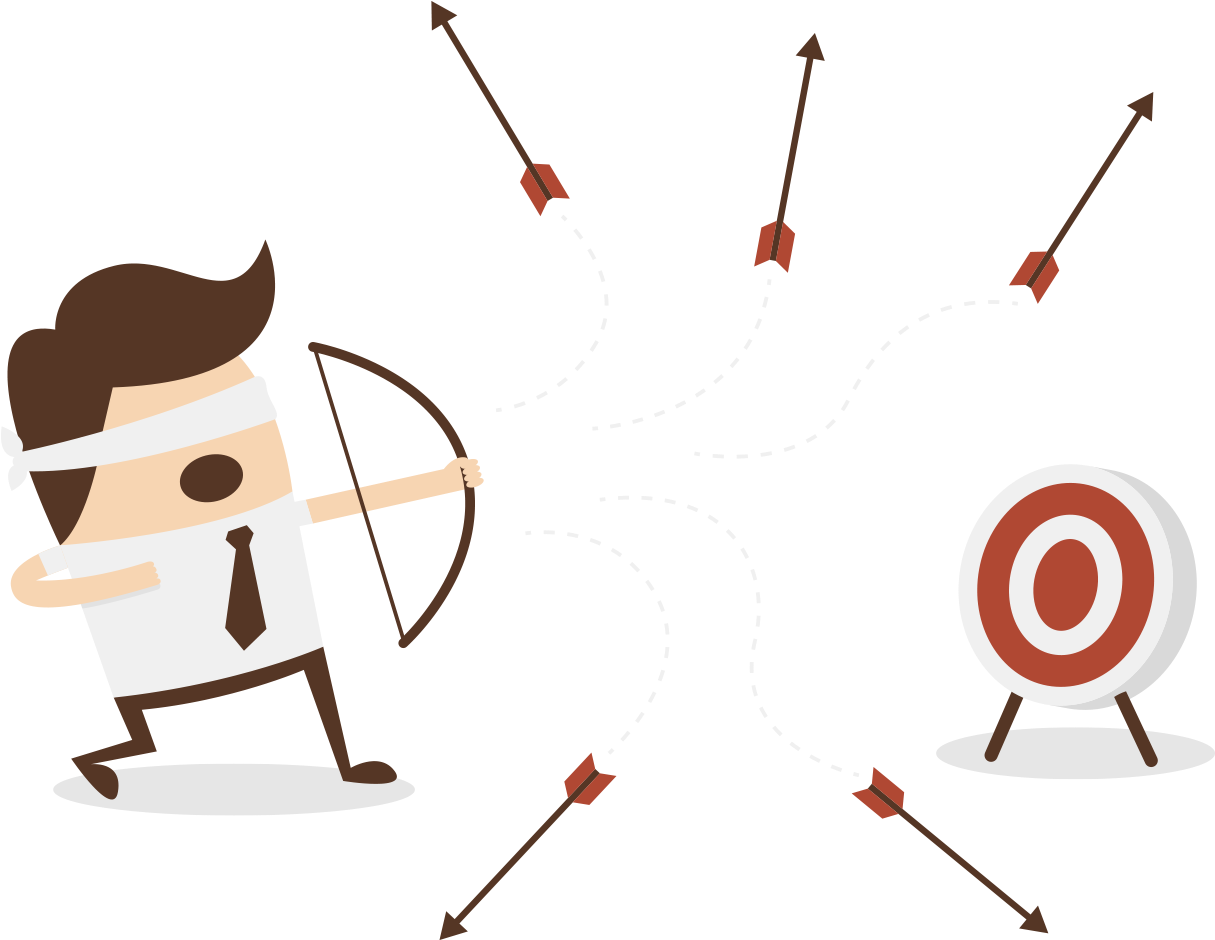
\includegraphics[width=1\textwidth,height=\textheight]{./pictures/clipart2906322_personal_use_only.png}}

}

\end{figure}

\bookmarksetup{startatroot}

\hypertarget{sec-vorwort}{%
\chapter*{Vorwort}\label{sec-vorwort}}
\addcontentsline{toc}{chapter}{Vorwort}

\markboth{Vorwort}{Vorwort}

Dieses Buch enthält Begleittexte und Übungsvorschläge für das
Studienfach \emph{Versprecher} (sl. \emph{Jezikovni spodrsljaji}, en.
\emph{speech errors}), das im Rahmen des Germanistikstudiums an der
Universität Maribor als Wahlfach angeboten wird.

Das Buch wurde mit Hilfe der Programmierungssprache \texttt{R}
\url{https://www.r-project.org/} und der von \texttt{RStudio}
\url{https://www.rstudio.com/} entwickelten Skriptsprache
\texttt{Rmarkdown} \url{https://rmarkdown.rstudio.com/} auf der
Entwickler-Platform \texttt{Github} \url{https://github.com/} als
\texttt{Quarto\ Book} \url{https://quarto.org/} veröffentlicht.

\part{Unbewusste Fehlleistungen}

\hypertarget{sec-einfuhrung}{%
\chapter{Einführung}\label{sec-einfuhrung}}

In diesem Buch besprechen wir verschiedene Arten von sprachlichen
Fehlleistungen und varietäten- bzw. textsortenbedingten Abweichungen von
der standardsprachlichen Norm im Deutschen (teilweise auch im
Slowenischen), die im Rahmen verschiedener Forschungsbereiche (Psycho-
und Neurolinguistik, Spracherwerb, Sprachvarietäten, \ldots) diskutiert
werden und auch für germanistische Studien von Interesse sein
können.\footnote{Dieses Buch wurde mit \texttt{Quarto}
  \url{https://quarto.org/docs/books/} zusammengestellt.}

Hinweise\footnote{Clipart von \url{https://www.clipartmax.com/}}:

Das ist eine Definition (rmdnote).

Das ist ein Tip oder eine Info (rmdtip).

Das ist ein Arbeitsvorschlag (rmdrobot).

Das ist der RStudio Logotyp (rmdrstudio).

Das ist eine Warnung (rmdwarning).

Das ist eine Fehlermeldung (rmderror).

\hypertarget{sec-gegenstand}{%
\chapter{Gegenstand}\label{sec-gegenstand}}

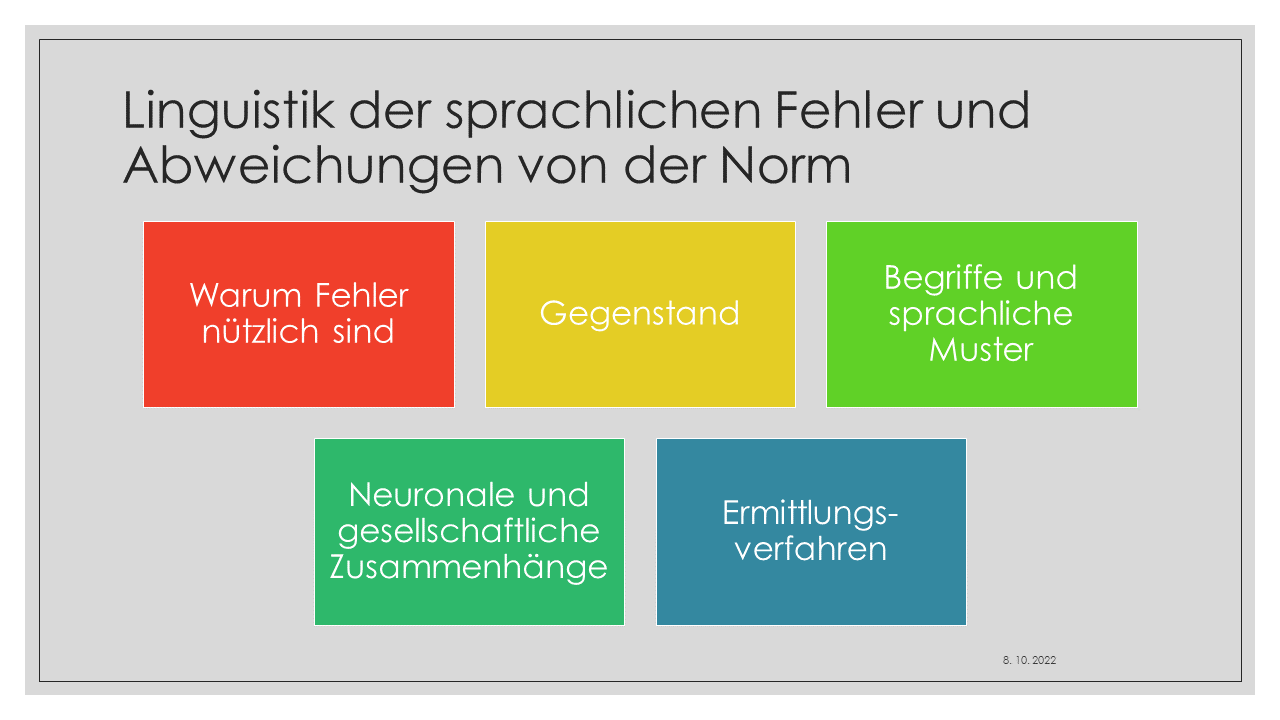
\includegraphics[width=1\textwidth,height=\textheight]{./pictures/Diapozitiv5.PNG}

In diesem Buch besprechen wir verschiedene Arten von sprachlichen
Fehlleistungen und varietäten- bzw. textsortenbedingten Abweichungen von
der standardsprachlichen Norm im Deutschen (teilweise auch im
Slowenischen), die im Rahmen verschiedener Forschungsbereiche (Psycho-
und Neurolinguistik, Spracherwerb, Sprachvarietäten, \ldots) diskutiert
werden und auch für germanistische Studien von Interesse sein können.
Berücksichtigt werden folgende sprachliche Erscheinungen:\\

\begin{itemize}
\tightlist
\item
  Zungenbrecher (en. tongue twisters, sl. lomilci jezika),\\
\item
  Zungenspitzen-Phänomen (en. tip of the tongue phenomenon, sl. izraz na
  konici jezika),\\
\item
  Versprecher (en. speech errors, spoonerisms, sl. jezikovni
  spodrsljaji),\\
\item
  sprachliche Fehler und Abweichungen im Spracherwerb (in diesem Buch
  mit Beschränkung auf den Erwerb der Zweit- und Fremdsprache),\\
\item
  Abweichungen von der standardsprachlichen Norm in neueren
  Kommunikationsformen (z.B. Chats, Sms, u.ä.),\\
\item
  Abweichungen von der standardsprachlichen Norm in multikulturellen
  Gemeinschaften (z.B. Kiezdeutsch),\\
\item
  und sprachliche Probleme und Fehlleistungen bei der Anwendung von
  gendergerechter Sprache (Ersatz des generischen Maskulinums durch
  potentielle Konkurrenzformen).\\
\end{itemize}

In diesem Einführungskurs machen wir Sie mit einigen der grundlegenden
Methoden zur Erfassung der linguistischen Merkmale in deutschen (und in
einigen Abschnitten auch mit slowenischen) Texten bekannt, in denen
diese sprachlichen Besonderheiten zu beobachten sind.

\hypertarget{sec-zungenbrecher}{%
\chapter{Zungenbrecher}\label{sec-zungenbrecher}}

\begin{figure}

{\centering 

\href{https://www.kissclipart.com/tongue-twister-cartoon-comics-stop-consonant-m2n92r/}{
\includegraphics[width=1\textwidth,height=\textheight]{./pictures/kissclipart-tongue-twister-cartoon-comics-stop-consonant-82fba1d0b8543744.png}}

}

\end{figure}

\hypertarget{was-sind-zungenbrecher}{%
\section{Was sind Zungenbrecher?}\label{was-sind-zungenbrecher}}

\emph{Zungenbrecher} (en. tongue twisters, sl. lomilci jezika), auch
zuweilen \emph{Lautüberfüllungen} genannt, sind ein bekanntes Phänomen
sowohl beim Erwerb einer Sprache als auch in der alltäglichen
Kommunikation, etwa in den öffentlichen Medien. Zungenbrecher sind
beliebt, werden von zahlreichen Sprachteilnehmern gesammelt und dienen
einerseits zur Belustigung oder Belebung eines Gesprächs oder des
Unterrichts, andererseits aber auch zu Schulungszwecken, da sie auch
beim Sprachtraining professioneller Mediensprecher von Nutzen sein
können.\footnote{https://de.wikipedia.org/wiki/Zungenbrecher}

17 Zungenbrecher innerhalb einer Minute von
\href{https://www.youtube.com/watch?v=VORRlhE7Hgk}{Rap Squad One}:

\{\{ \textless{} video src=https://www.youtube.com/watch?v=VORRlhE7Hgk/
title= ``17 Zungenbrecher in 1 Minute'' start=``1''
aspect-ratio=``16x9'' width=``100\%'' \textgreater{} \}\}

Bei Zungenbrechern handelt es sich um Lautfolgen, deren Aussprache nicht
nur Lernern einer fremden Sprache schwerfällt sondern auch
Erstsprachlern, insbesondere bei höherer Sprechgeschwindigkeit und auch
bei Wiederholungsversuchen zu Korrekturzwecken. Die Aussprache von
vielen Lautfolgen ist in der Erstsprache hochautomatisiert, so dass
gängige Lautkombinationen in sprachlichen Äußerungen gewöhnlich kein
Ausspracheproblem darstellen. Die Fehlerrate ist in der alltäglichen
sprachlichen Kommunikation gering. In sprachlichen Konstruktionen, die
sich als Zungenbrecher herausstellen, kommen jedoch ungewohnte
Wortabfolgen, ähnliche Laute und Silben oder Wörter, die sich
geringfügig voneinander unterscheiden, gehäuft vor. Diese Abweichungen
von gewohnten sprachlichen Konstruktionen erfordert erhöhte
Konzentration.

\hypertarget{zungenbrecher-typen}{%
\section{Zungenbrecher-Typen}\label{zungenbrecher-typen}}

Einige Zungenbrecher beruhen auf dem \emph{schnellen Wechsel}\\
- zwischen \emph{ähnlichen}, aber unterschiedlichen \emph{Phonemen}
(z.B. \textless s\textgreater{} {[}s{]} und \textless sch\textgreater{}
{[}ʃ{]} ),\\
- der Kombination von zwei verschiedenen Alternationsmustern,\\
- vertrauten Konstruktionen in Lehnwörtern\\
- oder anderen Merkmalen einer gesprochenen Sprache,\\
um schwer artikulierbar zu sein.

Zum Beispiel wurde der folgende Satz von William Poundstone als ``der
schwierigste der üblichen englischsprachigen Zungenbrecher''
bezeichnet.\footnote{https://en.wikipedia.org/wiki/Tongue\_twister}

\begin{tcolorbox}[enhanced jigsaw, colframe=quarto-callout-note-color-frame, toprule=.15mm, breakable, leftrule=.75mm, rightrule=.15mm, arc=.35mm, colback=white, left=2mm, bottomrule=.15mm, opacityback=0]
\begin{minipage}[t]{5.5mm}
\textcolor{quarto-callout-note-color}{\faInfo}
\end{minipage}%
\begin{minipage}[t]{\textwidth - 5.5mm}

\textbf{Beispiel}\vspace{2mm}

\emph{The seething sea ceaseth and thus the seething sea sufficeth
us.}\\
(Das brodelnde Meer hört auf zu brodeln, und so genügt uns das brodelnde
Meer.)

\end{minipage}%
\end{tcolorbox}

Diese absichtlich schwierigen Ausdrücke waren im 19. Jahrhundert sehr
beliebt. Der beliebte Zungenbrecher ``she sells seashells'' wurde
ursprünglich 1850 als Sprachübung veröffentlicht. Der Begriff
\emph{tongue twister} (Zungenbrecher) wurde erstmals 1895 für diese Art
von sprachlichen Ausdrücken verwendet.

Eine Reihe von Zungenbrechern verwendet eine Kombination aus
\emph{Alliteration} und \emph{Reim}. Sie bestehen aus zwei oder mehr
Lautfolgen, bei denen die Zunge zwischen den Silben neu positioniert
werden muss, dann werden dieselben Laute in einer anderen Reihenfolge
wiederholt.

\begin{tcolorbox}[enhanced jigsaw, colframe=quarto-callout-note-color-frame, toprule=.15mm, breakable, leftrule=.75mm, rightrule=.15mm, arc=.35mm, colback=white, left=2mm, bottomrule=.15mm, opacityback=0]
\begin{minipage}[t]{5.5mm}
\textcolor{quarto-callout-note-color}{\faInfo}
\end{minipage}%
\begin{minipage}[t]{\textwidth - 5.5mm}

\textbf{Beispiel}\vspace{2mm}

\emph{Fischers Fritze fischt frische Fische, frische Fische fischt
Fischers Fritze}

\end{minipage}%
\end{tcolorbox}

In anderen Zungenbrechern werden zusammengesetzte Wörter
(\emph{Komposita}) und ihre \emph{Stämme} genutzt, um die Artikulation
zu erschweren.

\begin{tcolorbox}[enhanced jigsaw, colframe=quarto-callout-note-color-frame, toprule=.15mm, breakable, leftrule=.75mm, rightrule=.15mm, arc=.35mm, colback=white, left=2mm, bottomrule=.15mm, opacityback=0]
\begin{minipage}[t]{5.5mm}
\textcolor{quarto-callout-note-color}{\faInfo}
\end{minipage}%
\begin{minipage}[t]{\textwidth - 5.5mm}

\textbf{Beispiel}\vspace{2mm}

\href{https://en.wikipedia.org/wiki/How_much_wood_would_a_woodchuck_chuck}{Woodchuck}\\
How much wood would a woodchuck chuck\\
if a woodchuck could chuck wood?\\
A woodchuck would chuck all the wood he could chuck\\
if a woodchuck would chuck wood.\\

\end{minipage}%
\end{tcolorbox}

Andere Zungenbrecher haben die Form eines Wortes oder \emph{kurzen
Phrase}, die sich bei schneller Wiederholung als Zungenbrecher
entpuppen.

\begin{tcolorbox}[enhanced jigsaw, colframe=quarto-callout-note-color-frame, toprule=.15mm, breakable, leftrule=.75mm, rightrule=.15mm, arc=.35mm, colback=white, left=2mm, bottomrule=.15mm, opacityback=0]
\begin{minipage}[t]{5.5mm}
\textcolor{quarto-callout-note-color}{\faInfo}
\end{minipage}%
\begin{minipage}[t]{\textwidth - 5.5mm}

\textbf{Beispiele}\vspace{2mm}

Neu-Schwanstein\\

Toy boat\\
Cricket critic\\
Unique New York\\
A proper copper coffee pot\\
Red leather, yellow leather\\
Irish wristwatch, Swiss wristwatch\\
Peggy Babcock\\

\end{minipage}%
\end{tcolorbox}

In manchen Fällen ergibt die inkorrekte Wiedergabe eines Spruchs einen
vulgären sprachlichen Ausdruck, was wiederum der Belustigung dient.

\begin{tcolorbox}[enhanced jigsaw, colframe=quarto-callout-note-color-frame, toprule=.15mm, breakable, leftrule=.75mm, rightrule=.15mm, arc=.35mm, colback=white, left=2mm, bottomrule=.15mm, opacityback=0]
\begin{minipage}[t]{5.5mm}
\textcolor{quarto-callout-note-color}{\faInfo}
\end{minipage}%
\begin{minipage}[t]{\textwidth - 5.5mm}

\textbf{Beispiele}\vspace{2mm}

\emph{Kaplan zdaj spi, zdaj je.}\\

Old Mother Hunt had a rough cut punt\\
Not a punt cut rough,\\
But a rough cut punt.\\

\end{minipage}%
\end{tcolorbox}

Einige Zungenbrecher wirken selbst bei korrekter Aussprache lustig:\\

\begin{tcolorbox}[enhanced jigsaw, colframe=quarto-callout-note-color-frame, toprule=.15mm, breakable, leftrule=.75mm, rightrule=.15mm, arc=.35mm, colback=white, left=2mm, bottomrule=.15mm, opacityback=0]
\begin{minipage}[t]{5.5mm}
\textcolor{quarto-callout-note-color}{\faInfo}
\end{minipage}%
\begin{minipage}[t]{\textwidth - 5.5mm}

\textbf{Beispiele}\vspace{2mm}

Are you copperbottoming those pans, my man?\\
No, I'm aluminiuming 'em Ma'am.\\
Pad kid poured curd pulled cold

\end{minipage}%
\end{tcolorbox}

\hypertarget{verwechselbare-phoneme}{%
\section{Verwechselbare Phoneme}\label{verwechselbare-phoneme}}

Die klangliche Ähnlichkeit und Artikulationsähnlichkeit von bestimmten
Sprachlauten scheint die Häufigkeit von sprachlichen Fehlleistungen zu
fördern.

Im Englischen werden die folgenden Phoneme häufig verwechselt:\\
- /l/ mit /r/ (z.B. \emph{lot}, \emph{rot}),\\
- /s/ mit /ʃ/ (z.B. \emph{sip}, \emph{ship}).\\
- /f/ mit /p/ (z.B. \emph{fit}, \emph{pit}),\\
- /w/ mit /r/ (z.B. \emph{which}, \emph{rich})\\
- u.a. laut einer MIT
Konfusionsmatrix\footnote{Wikipedia}(https://en.wikipedia.org/wiki/Tongue\_twister)

Bestimmte Phoneme sind \emph{schwieriger auszusprechen} als andere. Im
Englischen kann man davon ausgehen, dass {[}tʃ{]} wie im Anlaut von en.
\textless chair\textgreater{} schwieriger ist als ch {[}tʃ{]} wie in
\textless share\textgreater, was bei entsprechender Verteilung im Satz
einen Zungenbrecher heraufbeschwören
kann.\footnote{Wikipedia}(https://en.wikipedia.org/wiki/Tongue\_twister)
Dies führt gewöhnlich dazu, dass der schwierigere Laut durch den
einfacheren \emph{ersetzt} wird oder sogar \emph{getilgt} wird.
Entsprechendes gilt auch für Lenes (schwache Konsonanten) im Vergleich
zu Fortes (starken Konsonanten). \emph{Starke Konsonanten} (z.B. /ptk/
im Vergleich zu /bdg/) kommen in der Sprache häufiger vor, entwickeln
sich im Spracherwerb früher und bekommen in phonologischen
Phonemhierarchien Basispositionen zugewiesen. In Zungenbrechern werden
schwierigere Sprachlaute daher häufiger mit starken Konsonanten ersetzt.

Zungenbrecher sind sprachspezifisch. In bestimmten Sprachen können
beispielsweise auch die unterschiedliche Dauer von Vokalen oder
prosodische Unterschiede zwischen Silben eine Rolle bei der Entstehung
von Zungenbrechern spielen (etwa die Vokallänge).

--\textgreater{}
\href{https://en.wikipedia.org/wiki/Malapropism}{Malapropismus}: Texas
has a lot of electrical votes (electoral).\\
--\textgreater{}
\href{https://en.wikipedia.org/wiki/Spoonerism}{Spoonerismus}:
verwechselte Sprachlaute in Wörtern und Phrasen.\\
--\textgreater{}
\href{https://en.wikipedia.org/wiki/Shibboleth}{Shibboleth}: Wort oder
Phrase, die die Gruppenzugehörigkeit einer Person oder die Ausgrenzung
von sozialen Gruppen ermöglicht (z.B. aufgrund der Aussprache, die nur
von Einheimischen entsprechend realisiert wird und nicht von
Außenseitern oder Fremden).\\

In \emph{Hip-Hop oder Rap-Musiktexten} sind Zungenbrecher nicht selten.

Sprachliche Fehlleistungen wie die Zungenbrecher sind nicht nur auf die
Lautsprache beschränkt, sondern auch in der Gebärdensprache beobachtbar
(z.B. \emph{Vergebärdler}).

\hypertarget{erkluxe4rungsversuche}{%
\section{Erklärungsversuche}\label{erkluxe4rungsversuche}}

Was ist die \emph{Ursache} für aussprachebedingte sprachliche
Fehlleistungen?

Außer artikulatorischer und klanglicher Ähnlichkeit scheint die
Ähnlichkeit der Muskelbewegungen und ihre Repräsentation im Gehirn eine
Rolle bei der Entstheung von sprachlichen Fehlleistungen wie den
Zungenbrechern zu spielen.

Erkärungsversuch, veröffentlicht in der wissenschaftlichen Zeitschrift
\href{https://www.nature.com/articles/nature.2013.12471.pdf}{Nature}:\\

Ausgefeilte mehrdimensionale statistische Verfahren ermöglichten es den
Forschern, die riesigen Datenmengen zu sichten und aufzudecken wie
grundlegende neuronale Bausteine -- Muster von Neuronen, die im Laufe
der Zeit an verschiedenen Orten feuern -- sich kombinieren, um die
Sprachlaute des Amerikanischen Englischs zu bilden.

Die Muster für \emph{Konsonanten} waren ganz \emph{anders} als für
\emph{Vokale}, auch wenn die Sprechlaute genau die \emph{gleichen Teile
des Vokaltrakts nutzen}, sagt der Autor Edward Chang, ein
Neurowissenschaftler an der University of California in San Francisco.

\emph{Die Lippen, die Zähne, die Zungenspitze}

Die verschiedenen Muster könnten helfen zu erklären, warum
\emph{Versprecher} auf vorhersehbare Weise auftreten: Wir vertauschen
oft zwei Konsonanten in sogenannte \emph{Spoonerismen} (en. `Boat-Tag'
statt en. `Tote Bag') oder verwechseln zwei Vokale (`wheel' (Rad) für
`whale' Wal), tauschen aber \emph{selten Konsonanten gegen Vokale} aus.4

Das Team fand auch heraus, dass das Gehirn die Artikulation anscheinend
nicht nach dem \emph{Klang} der resultierenden Phoneme koordiniert, wie
bisher vermutet, sondern wie sich die \emph{Muskeln bewegen} müssen.

\begin{tcolorbox}[enhanced jigsaw, colframe=quarto-callout-important-color-frame, bottomtitle=1mm, toprule=.15mm, titlerule=0mm, leftrule=.75mm, rightrule=.15mm, title=\textcolor{quarto-callout-important-color}{\faExclamation}\hspace{0.5em}{Phonemkategorien (nach Muskelbewegungen)}, colback=white, left=2mm, coltitle=black, toptitle=1mm, breakable, colbacktitle=quarto-callout-important-color!10!white, arc=.35mm, bottomrule=.15mm, opacitybacktitle=0.6, opacityback=0]

Die Daten ergaben \emph{drei Kategorien von Konsonanten}:\\
- koronale Konsonanten, ausgesprochen mit dem vorderen Zungenrand (wie
/z/ im Anlaut des Wortes \textless Seife\textgreater{} ),\\
- velare Konsonanten, ausgesprochen mit dem hinteren Zungenblatt (wie
/g/ im Anlaut des Wortes \textless Gas\textgreater{} ) und\\
- labiale Konstonanten, ausgesprochen mit den Lippen (wie /m/ im Anlaut
des Wortes \textless Mus\textgreater{} ).

\emph{Vokale} teilen sich in \emph{zwei Gruppen} auf:\\
- gerundete Vokale (wie /u/ in \textless Lu-pe\textgreater{} ) und\\
- ungerundete Vokale (wie /a/ in \textless La-de\textgreater{} ).

\end{tcolorbox}

Das impliziert, dass \emph{Zungenbrecher} harte Aussprachebrocken sind,
weil sich (laut Chang) ``die \emph{Repräsentationen} im Gehirn stark
\emph{überlappen}''.

\begin{tcolorbox}[enhanced jigsaw, colframe=quarto-callout-note-color-frame, toprule=.15mm, breakable, leftrule=.75mm, rightrule=.15mm, arc=.35mm, colback=white, left=2mm, bottomrule=.15mm, opacityback=0]
\begin{minipage}[t]{5.5mm}
\textcolor{quarto-callout-note-color}{\faInfo}
\end{minipage}%
\begin{minipage}[t]{\textwidth - 5.5mm}

\textbf{Beispiel}\vspace{2mm}

Zum Beispiel werden `/s/' und `/š/' beide im Gehirn als
Front-of-the-Tongue-Sounds (\emph{koronale} Laute) gespeichert, so dass
das Gehirn diese wahrscheinlich \emph{häufiger verwechselt} als Laute,
die von \emph{verschiedenen Teilen} der Zunge bzw. Sprechwerkzeuge
gebildet werden (z.B. /s/ vs.~/m/).

\end{minipage}%
\end{tcolorbox}

\begin{tcolorbox}[enhanced jigsaw, colframe=quarto-callout-note-color-frame, toprule=.15mm, breakable, leftrule=.75mm, rightrule=.15mm, arc=.35mm, colback=white, left=2mm, bottomrule=.15mm, opacityback=0]
\begin{minipage}[t]{5.5mm}
\textcolor{quarto-callout-note-color}{\faInfo}
\end{minipage}%
\begin{minipage}[t]{\textwidth - 5.5mm}

\textbf{Beispiel}\vspace{2mm}

\emph{Sally sells seashells} (Sally verkauft Muscheln) ist knifflig.\\
\emph{Mally sells sea-smells} (Mally verkauft Meeresgerüche) ist es
nicht.

\end{minipage}%
\end{tcolorbox}

\begin{enumerate}
\def\labelenumi{\arabic{enumi}.}
\tightlist
\item
  Öffnen Sie die Video-Datei auf YouTube
  (https://www.youtube.com/watch?v=wuK\_znJRKhU) mit 11 schwierigen
  Sprüchen auf Ihrem Computer -- und stoppen Sie die Wiedergabe.\\
\item
  Öffnen Sie ein Programm zur Aufnahme Ihrer Stimme (Praat, Windows
  Recorder, Audacity, Sony Soloist \ldots), setzen Sie Ihr Headset
  (Kopfhörer mit Mikrofon) auf und drücken Sie Aufnahme.\\
\item
  Spielen Sie die bereits geöffnete Video-Datei mit den elf deutschen
  Zungenbrechern ab.\\
\item
  Lesen Sie die Zungenbrecher nacheinander vom Bildschirm ab, sprechen
  sie diesen möglichst schnell und ohne Fehler ins Mikrofon. Die Zeit
  für jeden Zungenbrecher ist beschränkt. Jeder der elf Zungenbrecher
  soll von Ihnen vollständig ausgesprochen werden. Gewöhnlich werten wir
  den ersten Durchgang für die folgende Analyse. Wiederholen Sie
  eventuell nur diejenigen Zungenbrecher, die Sie nicht zu Ende
  ausgesprochen haben (z.B. wegen Zeitmangel oder weil Sie verwirrt
  waren).\\
\item
  Laden Sie Ihre Aufnahme als erste Aufgabe (assignment) hoch (Aufgabe
  N01).\\
\end{enumerate}

Ihre nächste Aufgabe wird darin bestehen, die in Ihrer Aufnahme
gemachten sprachlichen Fehlleistungen zu identifizieren und in Klassen
einzuordnen.

\hypertarget{sec-zungenspitze}{%
\chapter{Zungenspitzen-Phänomen}\label{sec-zungenspitze}}

\hypertarget{sec-versprecher}{%
\chapter{Versprecher}\label{sec-versprecher}}

\part{Normabweichungen und Normwandel}

\hypertarget{sec-spracherwerb}{%
\chapter{Fehler im Spracherwerb}\label{sec-spracherwerb}}

Fehler in Zweit- und Fremdsprache

\hypertarget{sec-medien}{%
\chapter{Normabweichungen in den neuen Medien}\label{sec-medien}}

\hypertarget{sec-multikulti}{%
\chapter{Multikulturelle Sprachvarietäten}\label{sec-multikulti}}

Kiezdeutsch als Beispiel für Abweichungen von der standardsprachlichen
Norm mit der Entwicklung einer varietätenspezifischen Grammatik.

\hypertarget{sec-gender}{%
\chapter{Gendergerechte Sprache}\label{sec-gender}}

Fehler und Abweichungen beim Bezug auf verschiedene Geschlechter,
insbesondere bei der Vermeidung des generischen Maskulinums.

\bookmarksetup{startatroot}

\hypertarget{abschlieuxdfende-bemerkungen}{%
\chapter{Abschließende Bemerkungen}\label{abschlieuxdfende-bemerkungen}}

Einige Hinweise für \emph{\texttt{selbständige}} Textanalysen. 🤗

\{\{ \textless{} include \_WM\_Presentation.qmd \textgreater{} \}\}

\hypertarget{callout-types}{%
\section{Callout Types}\label{callout-types}}

\begin{tcolorbox}[enhanced jigsaw, colframe=quarto-callout-note-color-frame, bottomtitle=1mm, toprule=.15mm, titlerule=0mm, leftrule=.75mm, rightrule=.15mm, title=\textcolor{quarto-callout-note-color}{\faInfo}\hspace{0.5em}{Note}, colback=white, left=2mm, coltitle=black, toptitle=1mm, breakable, colbacktitle=quarto-callout-note-color!10!white, arc=.35mm, bottomrule=.15mm, opacitybacktitle=0.6, opacityback=0]

Note that there are five types of callouts, including: \texttt{note},
\texttt{warning}, \texttt{important}, \texttt{tip}, and
\texttt{caution}.

\end{tcolorbox}

\begin{tcolorbox}[enhanced jigsaw, colframe=quarto-callout-tip-color-frame, bottomtitle=1mm, toprule=.15mm, titlerule=0mm, leftrule=.75mm, rightrule=.15mm, title=\textcolor{quarto-callout-tip-color}{\faLightbulb}\hspace{0.5em}{Tip With Caption / Tipp mit Titel}, colback=white, left=2mm, coltitle=black, toptitle=1mm, breakable, colbacktitle=quarto-callout-tip-color!10!white, arc=.35mm, bottomrule=.15mm, opacitybacktitle=0.6, opacityback=0]

This is an example of a callout with a caption.

\end{tcolorbox}

\begin{tcolorbox}[enhanced jigsaw, colframe=quarto-callout-important-color-frame, bottomtitle=1mm, toprule=.15mm, titlerule=0mm, leftrule=.75mm, rightrule=.15mm, title=\textcolor{quarto-callout-important-color}{\faExclamation}\hspace{0.5em}{Important}, colback=white, left=2mm, coltitle=black, toptitle=1mm, breakable, colbacktitle=quarto-callout-important-color!10!white, arc=.35mm, bottomrule=.15mm, opacitybacktitle=0.6, opacityback=0]

Das ist wichtig.

\end{tcolorbox}

\begin{tcolorbox}[enhanced jigsaw, colframe=quarto-callout-warning-color-frame, bottomtitle=1mm, toprule=.15mm, titlerule=0mm, leftrule=.75mm, rightrule=.15mm, title=\textcolor{quarto-callout-warning-color}{\faExclamationTriangle}\hspace{0.5em}{Warning}, colback=white, left=2mm, coltitle=black, toptitle=1mm, breakable, colbacktitle=quarto-callout-warning-color!10!white, arc=.35mm, bottomrule=.15mm, opacitybacktitle=0.6, opacityback=0]

Warning

\end{tcolorbox}

\begin{tcolorbox}[enhanced jigsaw, colframe=quarto-callout-caution-color-frame, bottomtitle=1mm, toprule=.15mm, titlerule=0mm, leftrule=.75mm, rightrule=.15mm, title=\textcolor{quarto-callout-caution-color}{\faFire}\hspace{0.5em}{Expand To Learn About Collapse}, colback=white, left=2mm, coltitle=black, toptitle=1mm, breakable, colbacktitle=quarto-callout-caution-color!10!white, arc=.35mm, bottomrule=.15mm, opacitybacktitle=0.6, opacityback=0]

This is an example of a `folded' caution callout that can be expanded by
the user. You can use \texttt{collapse="true"} to collapse it by default
or \texttt{collapse="false"} to make a collapsible callout that is
expanded by default.

\end{tcolorbox}

\hypertarget{diagrammer-mermaid}{%
\section{DiagrammeR mermaid}\label{diagrammer-mermaid}}

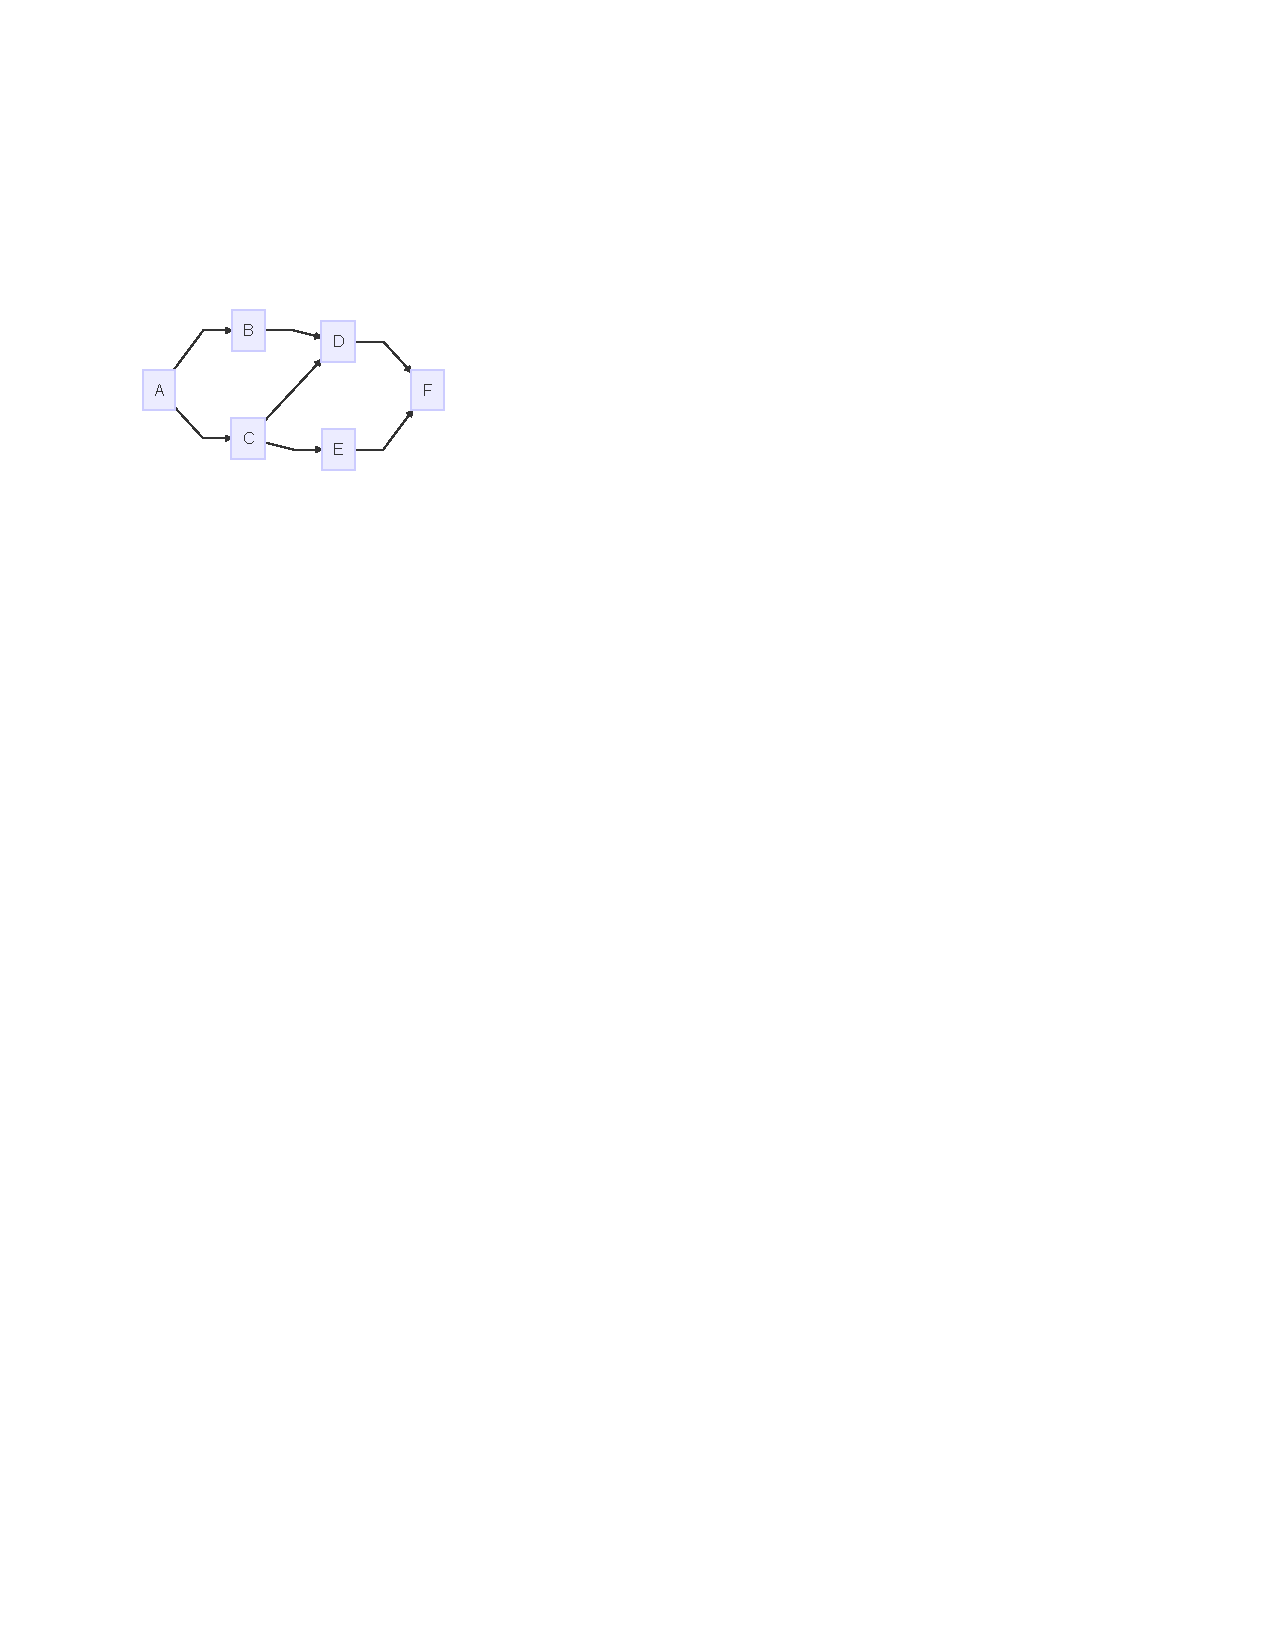
\includegraphics{./summary_files/figure-pdf/unnamed-chunk-1-1.pdf}

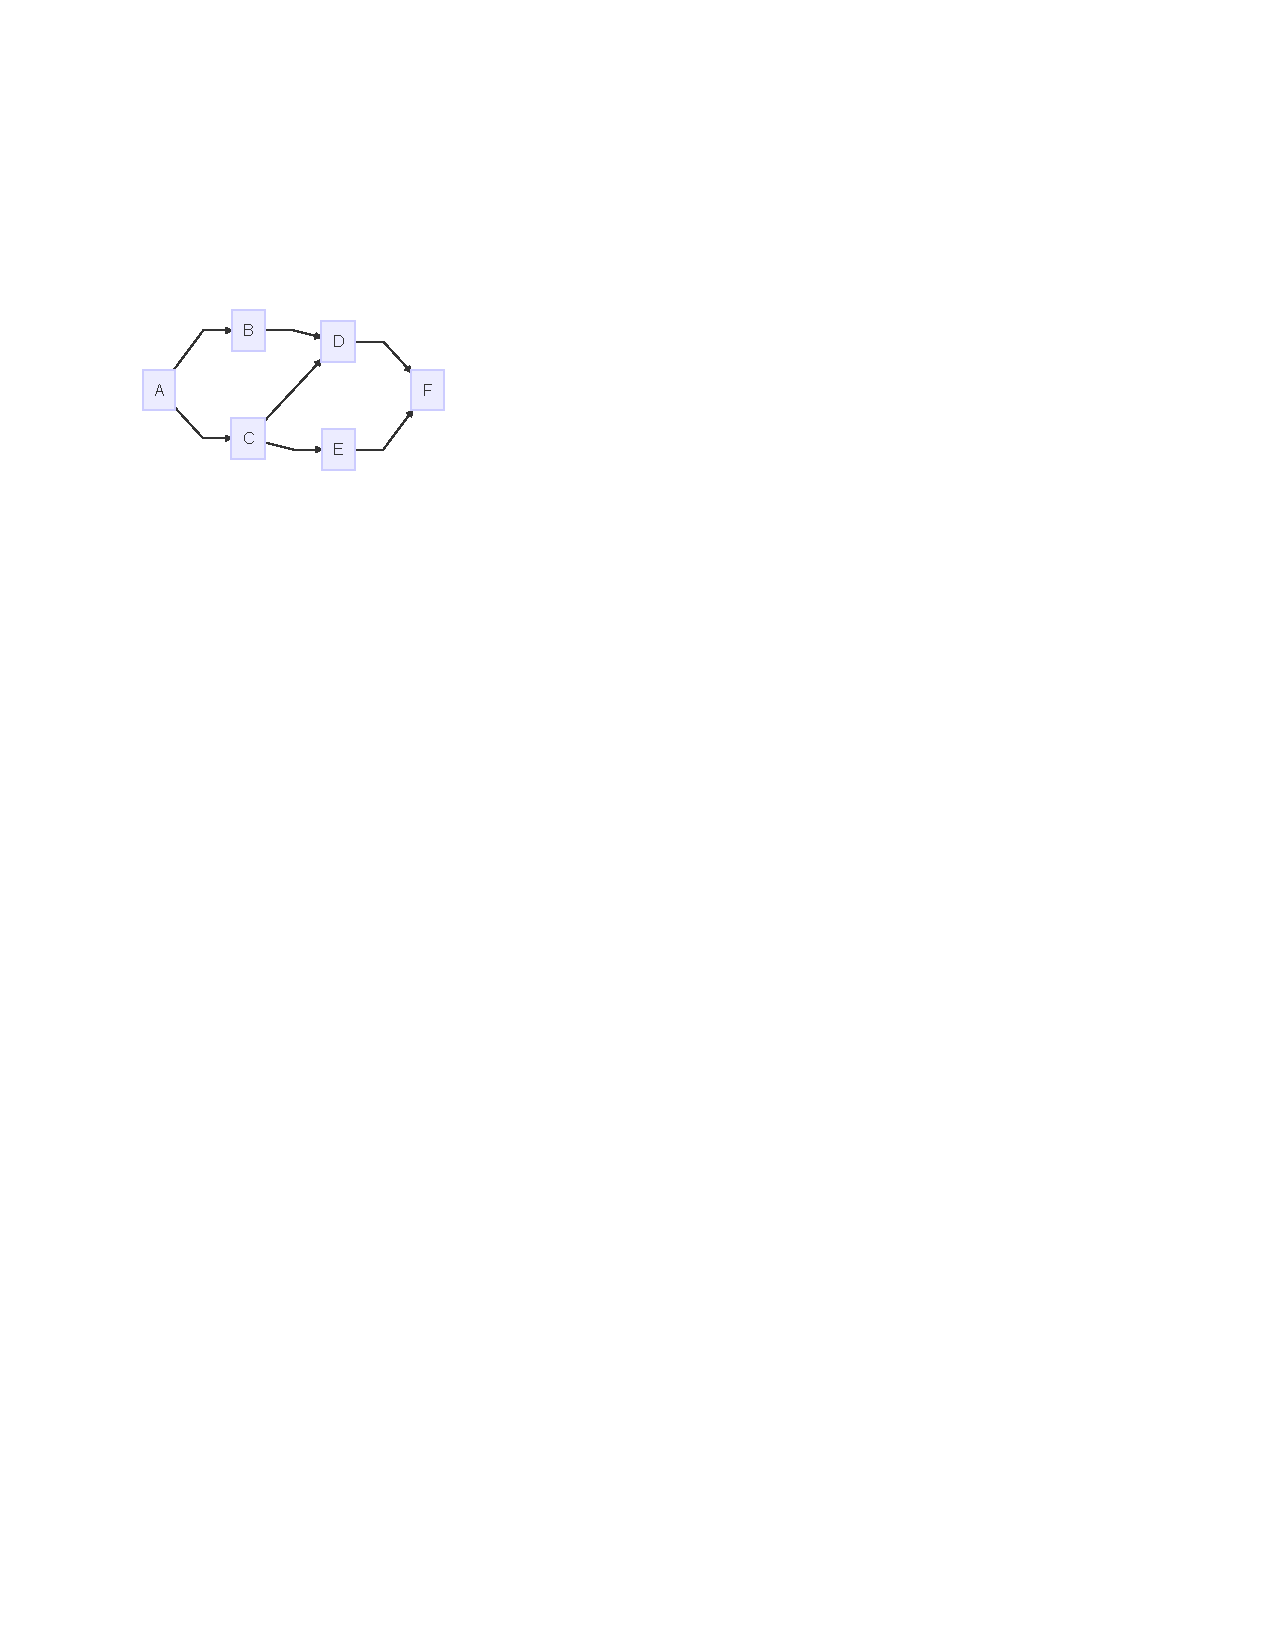
\includegraphics{./summary_files/figure-pdf/unnamed-chunk-2-1.pdf}

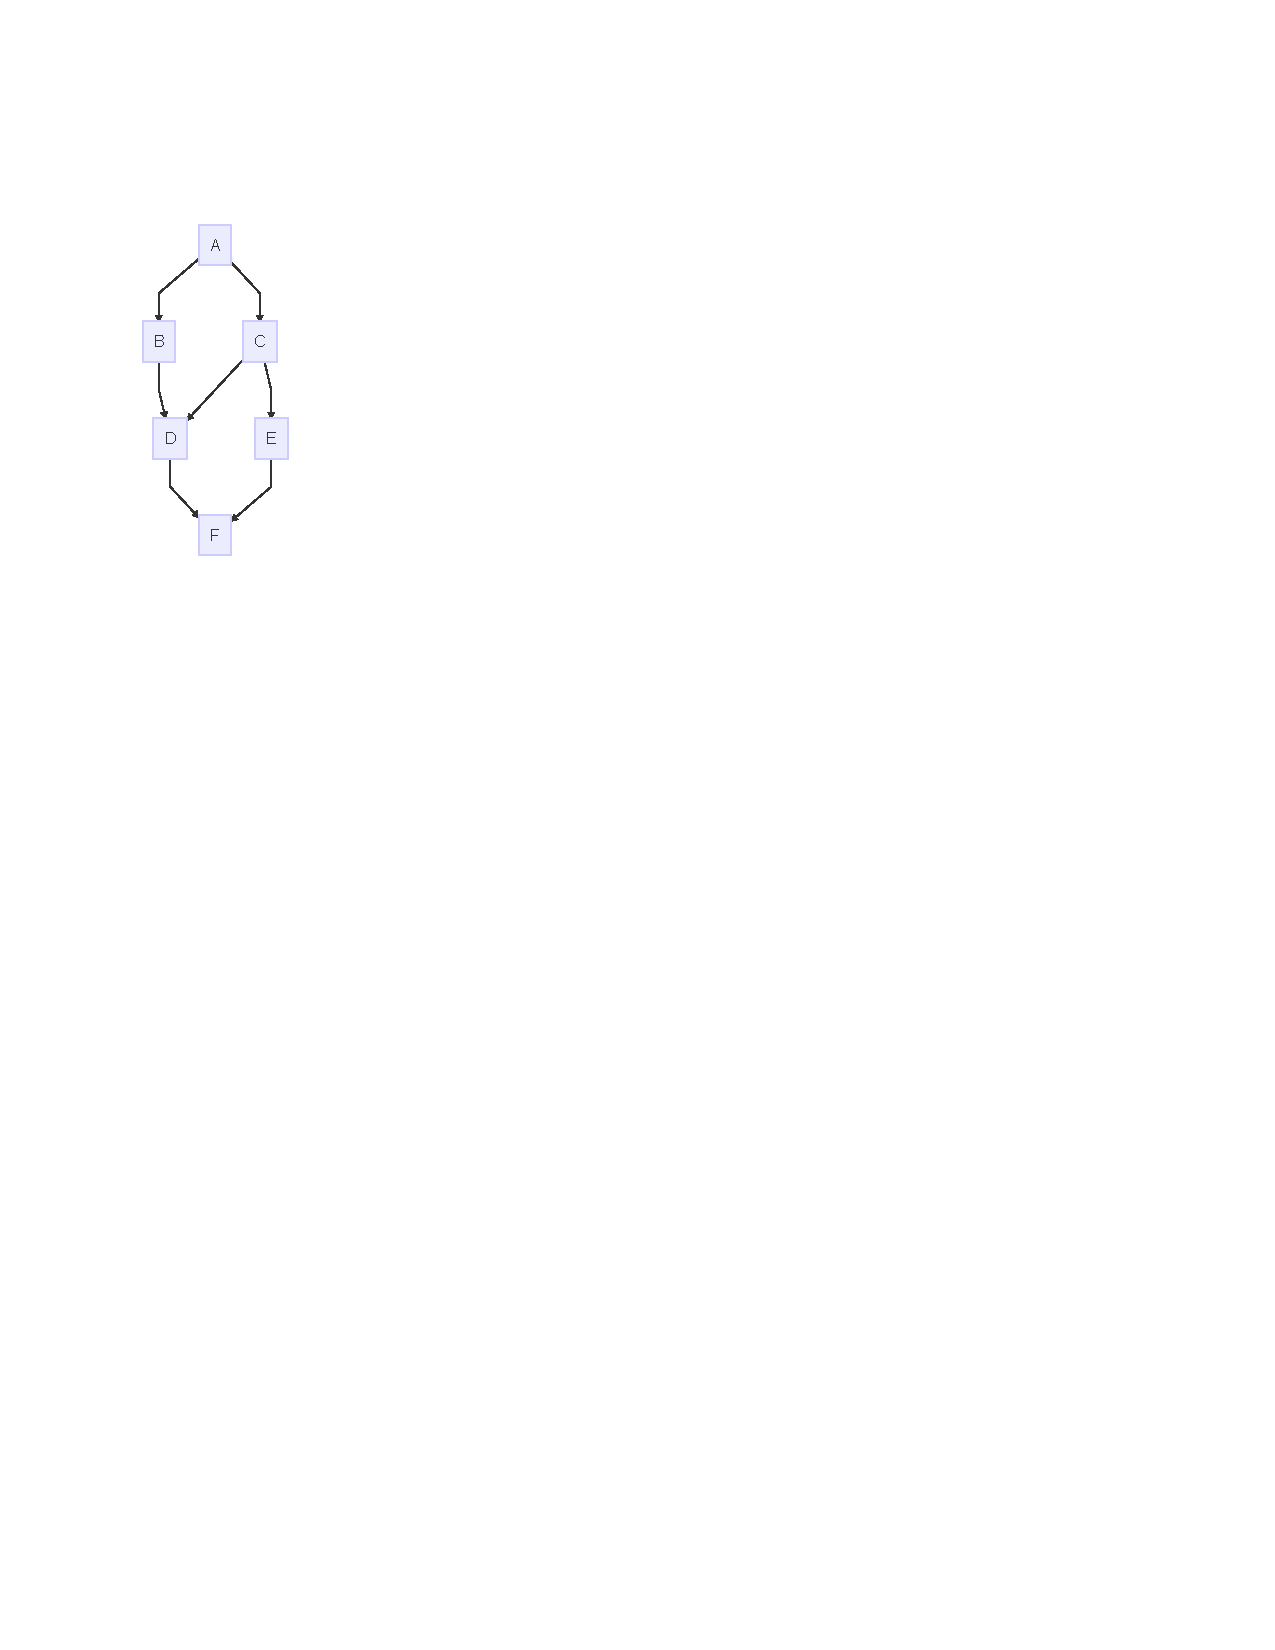
\includegraphics{./summary_files/figure-pdf/unnamed-chunk-3-1.pdf}

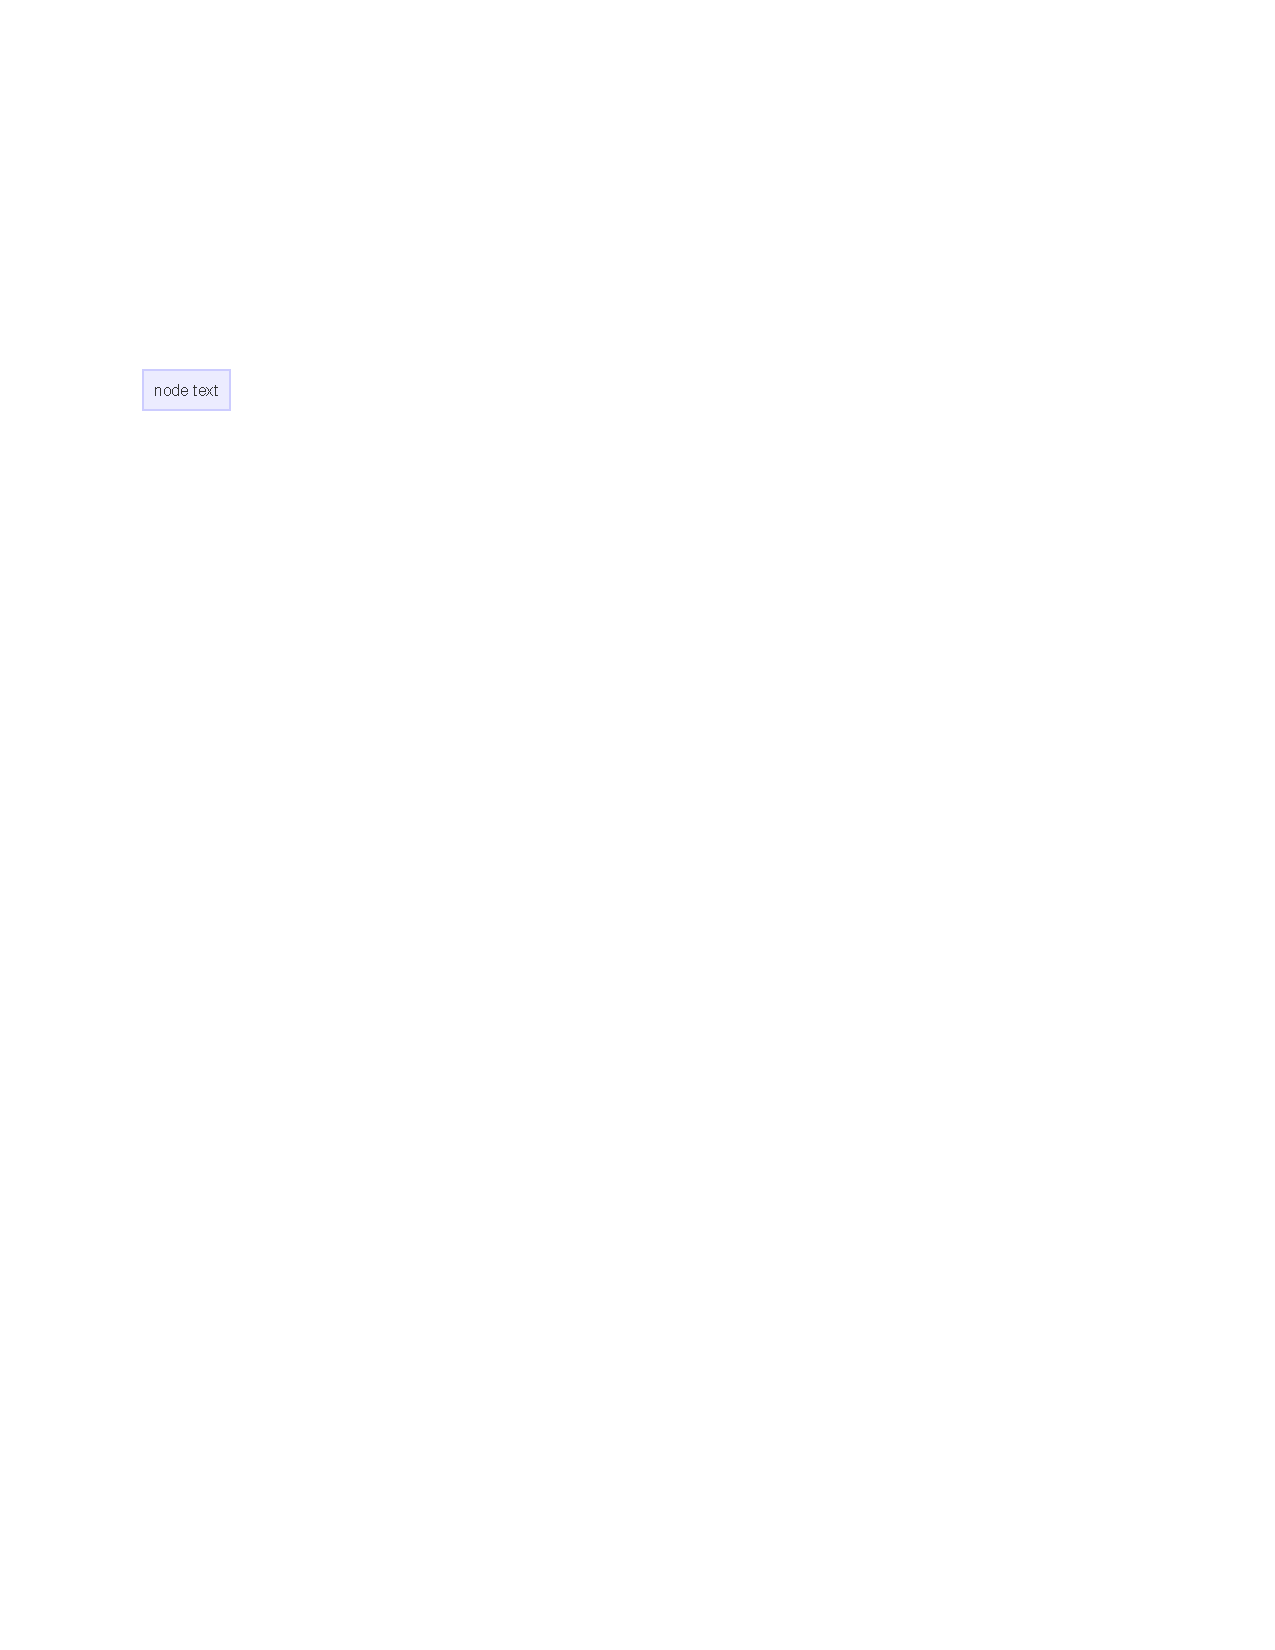
\includegraphics{./summary_files/figure-pdf/unnamed-chunk-4-1.pdf}

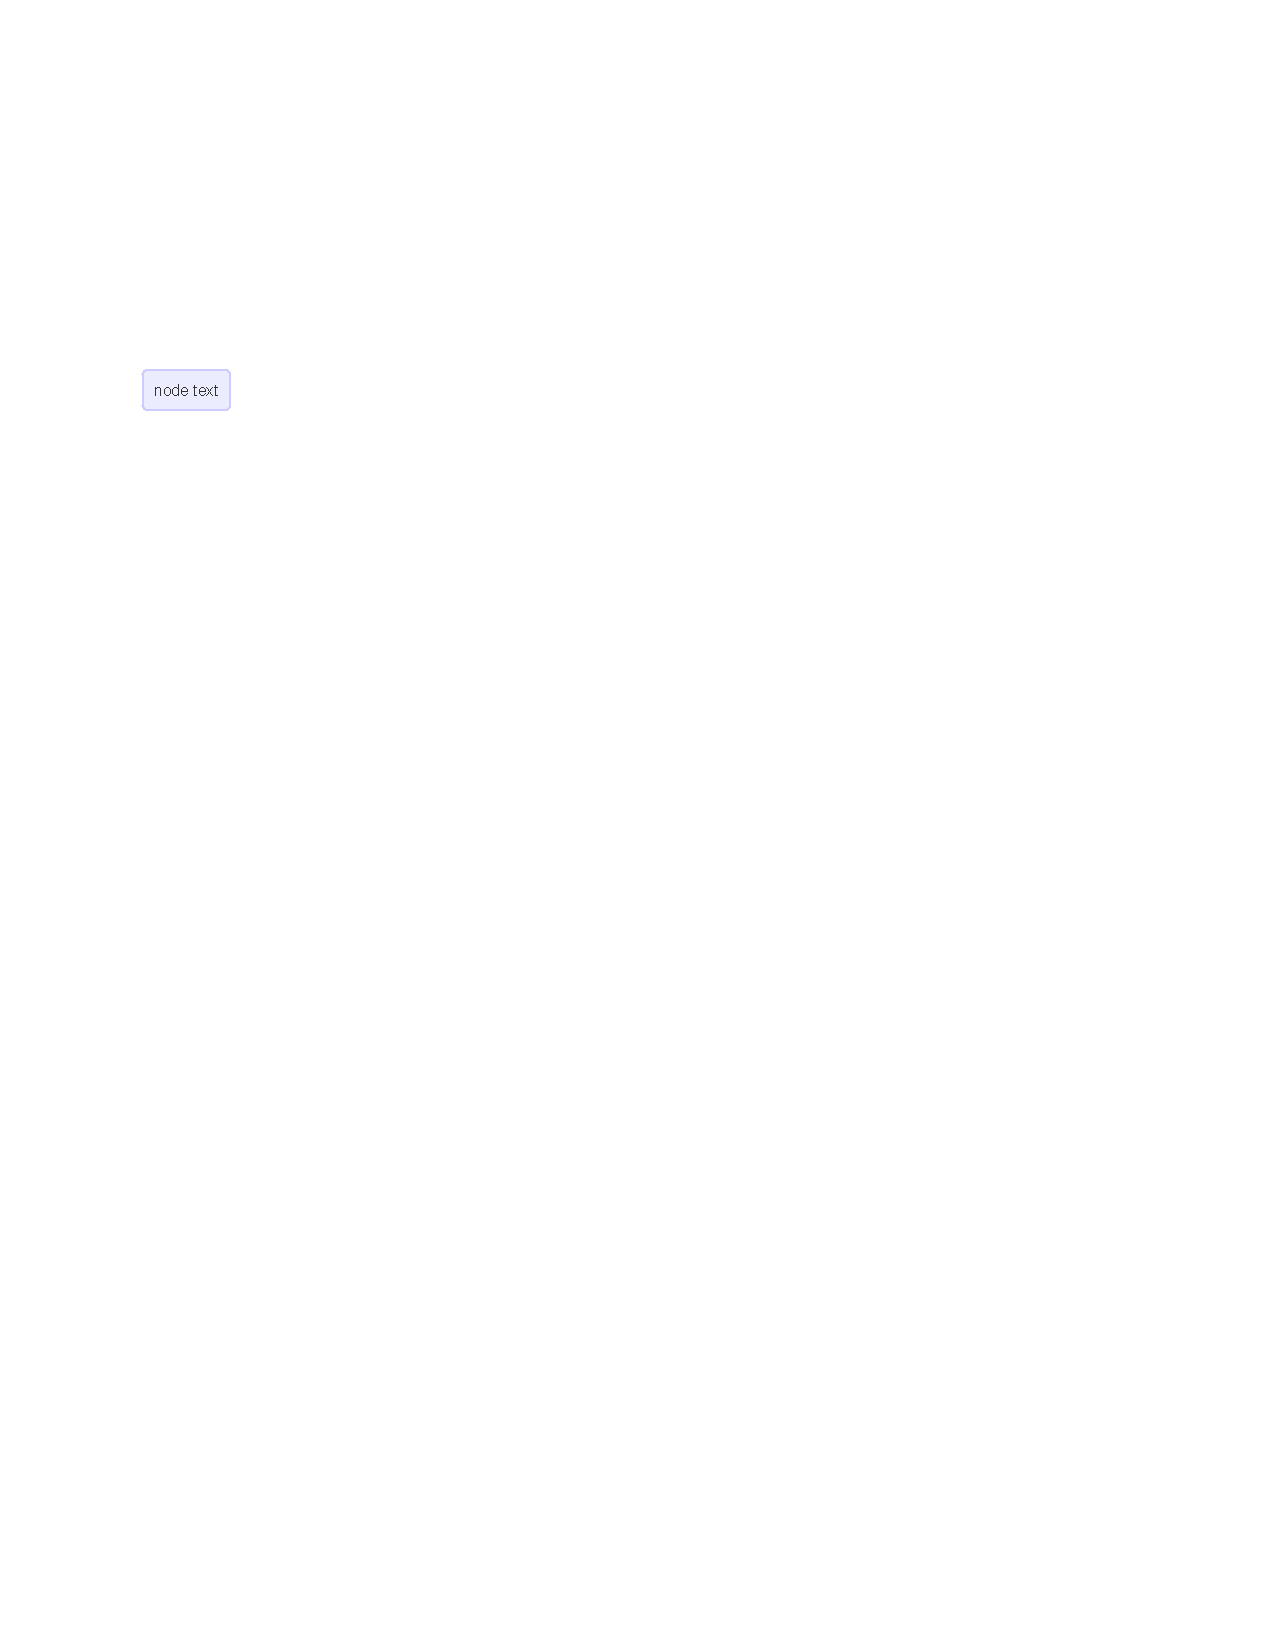
\includegraphics{./summary_files/figure-pdf/unnamed-chunk-4-2.pdf}

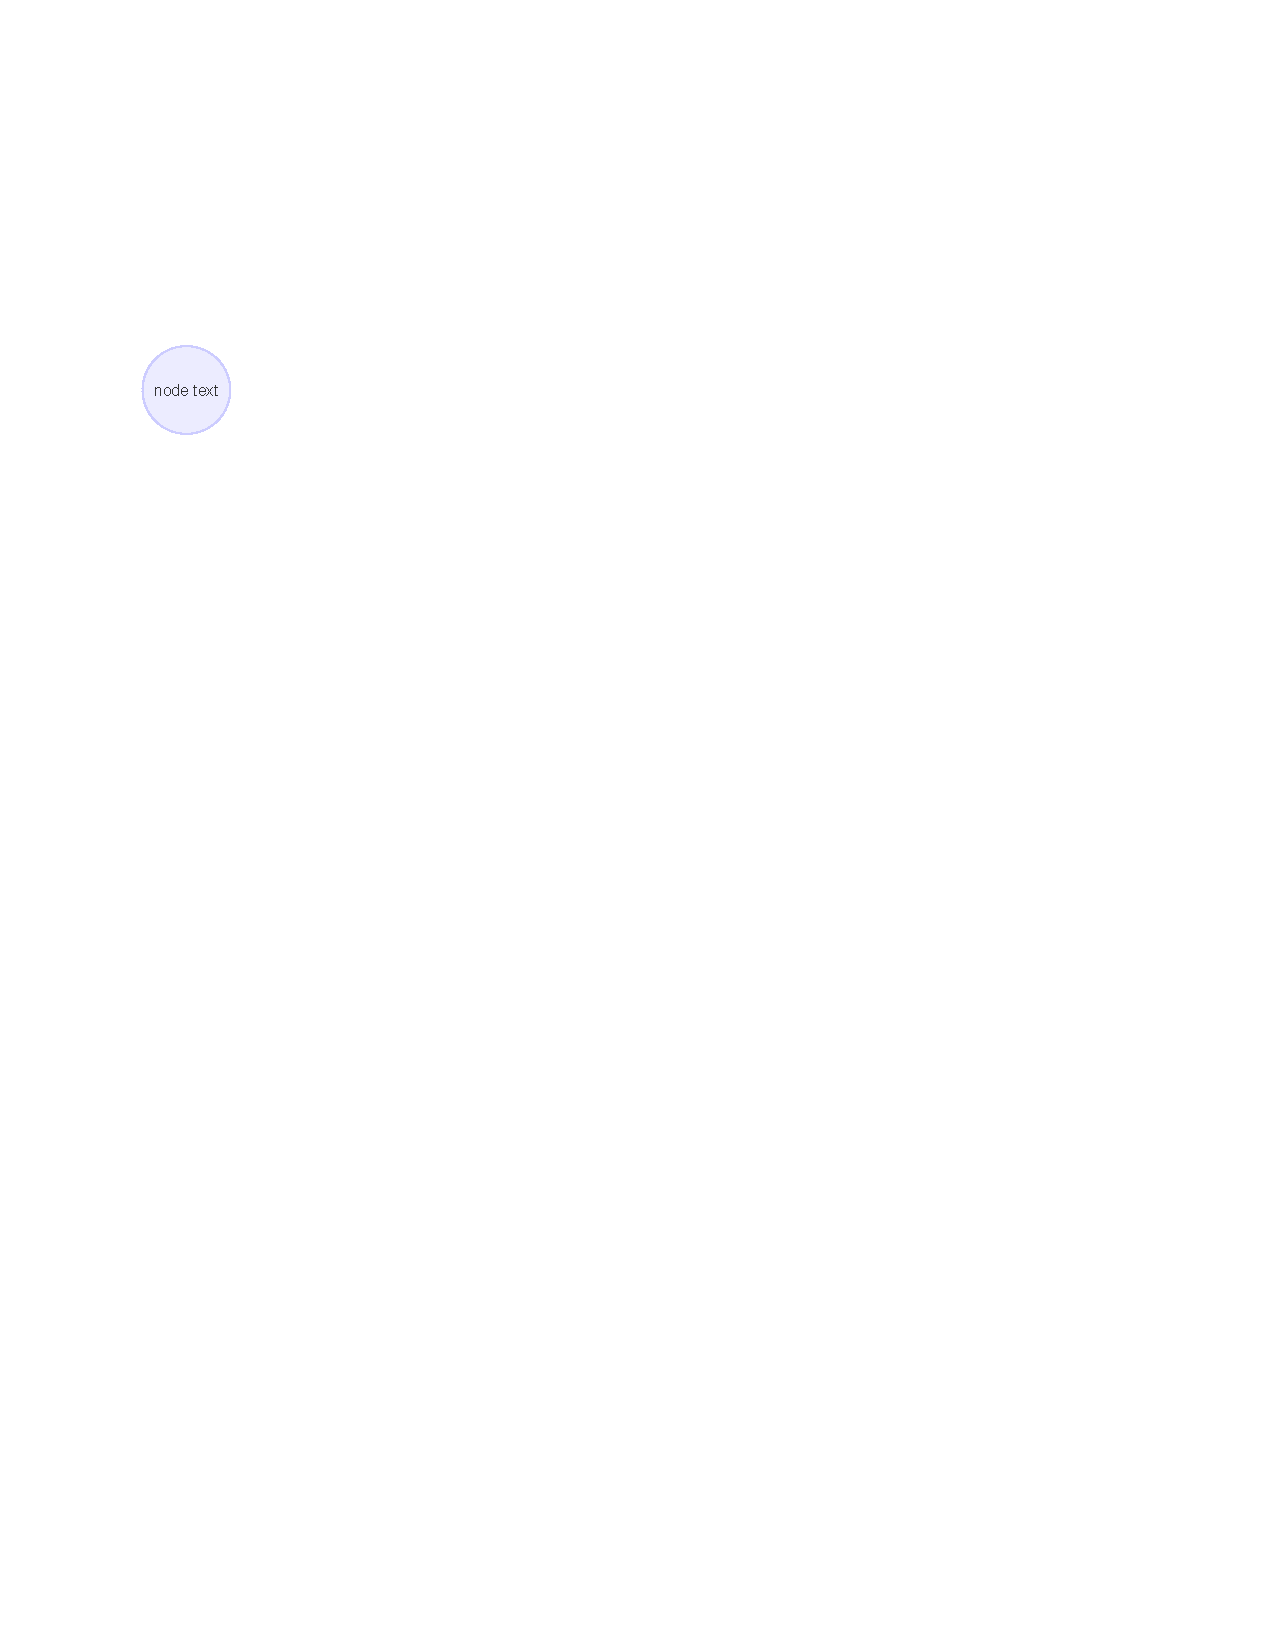
\includegraphics{./summary_files/figure-pdf/unnamed-chunk-4-3.pdf}

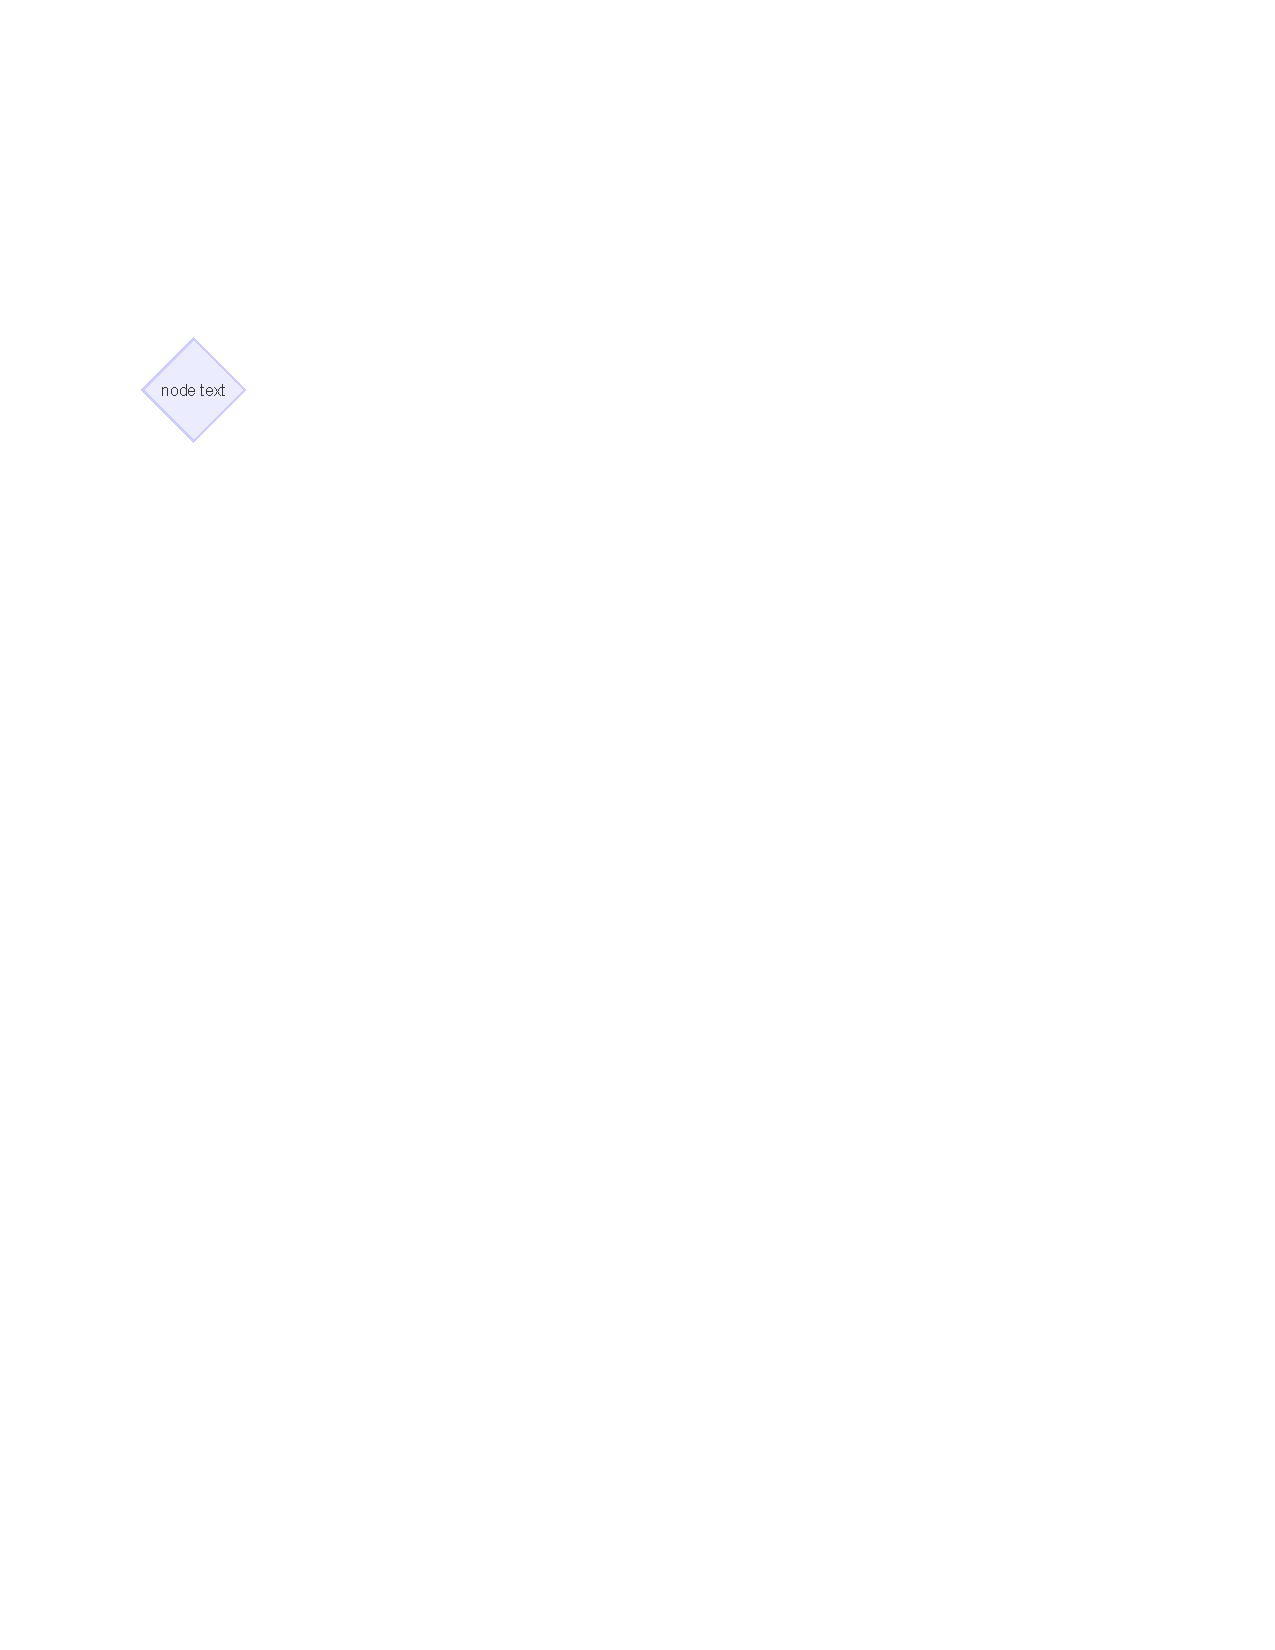
\includegraphics{./summary_files/figure-pdf/unnamed-chunk-4-4.pdf}

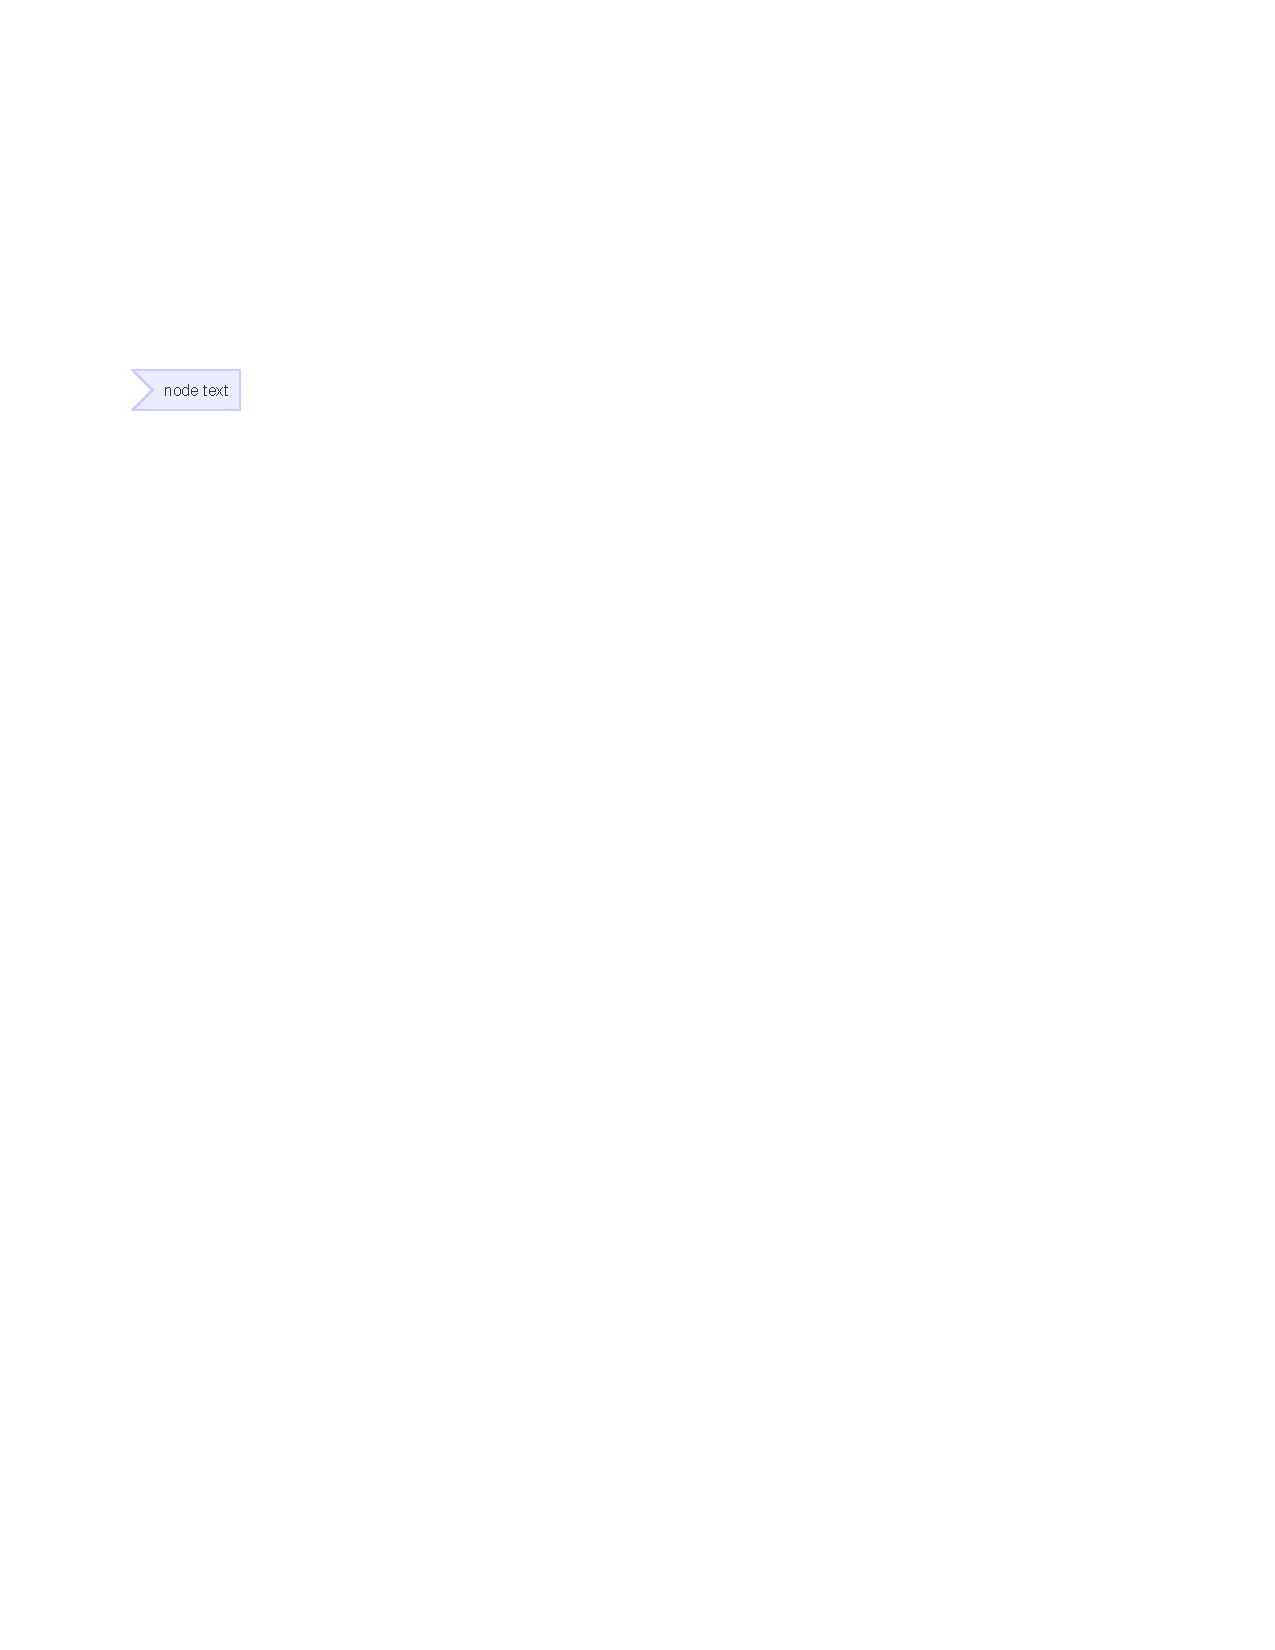
\includegraphics{./summary_files/figure-pdf/unnamed-chunk-4-5.pdf}

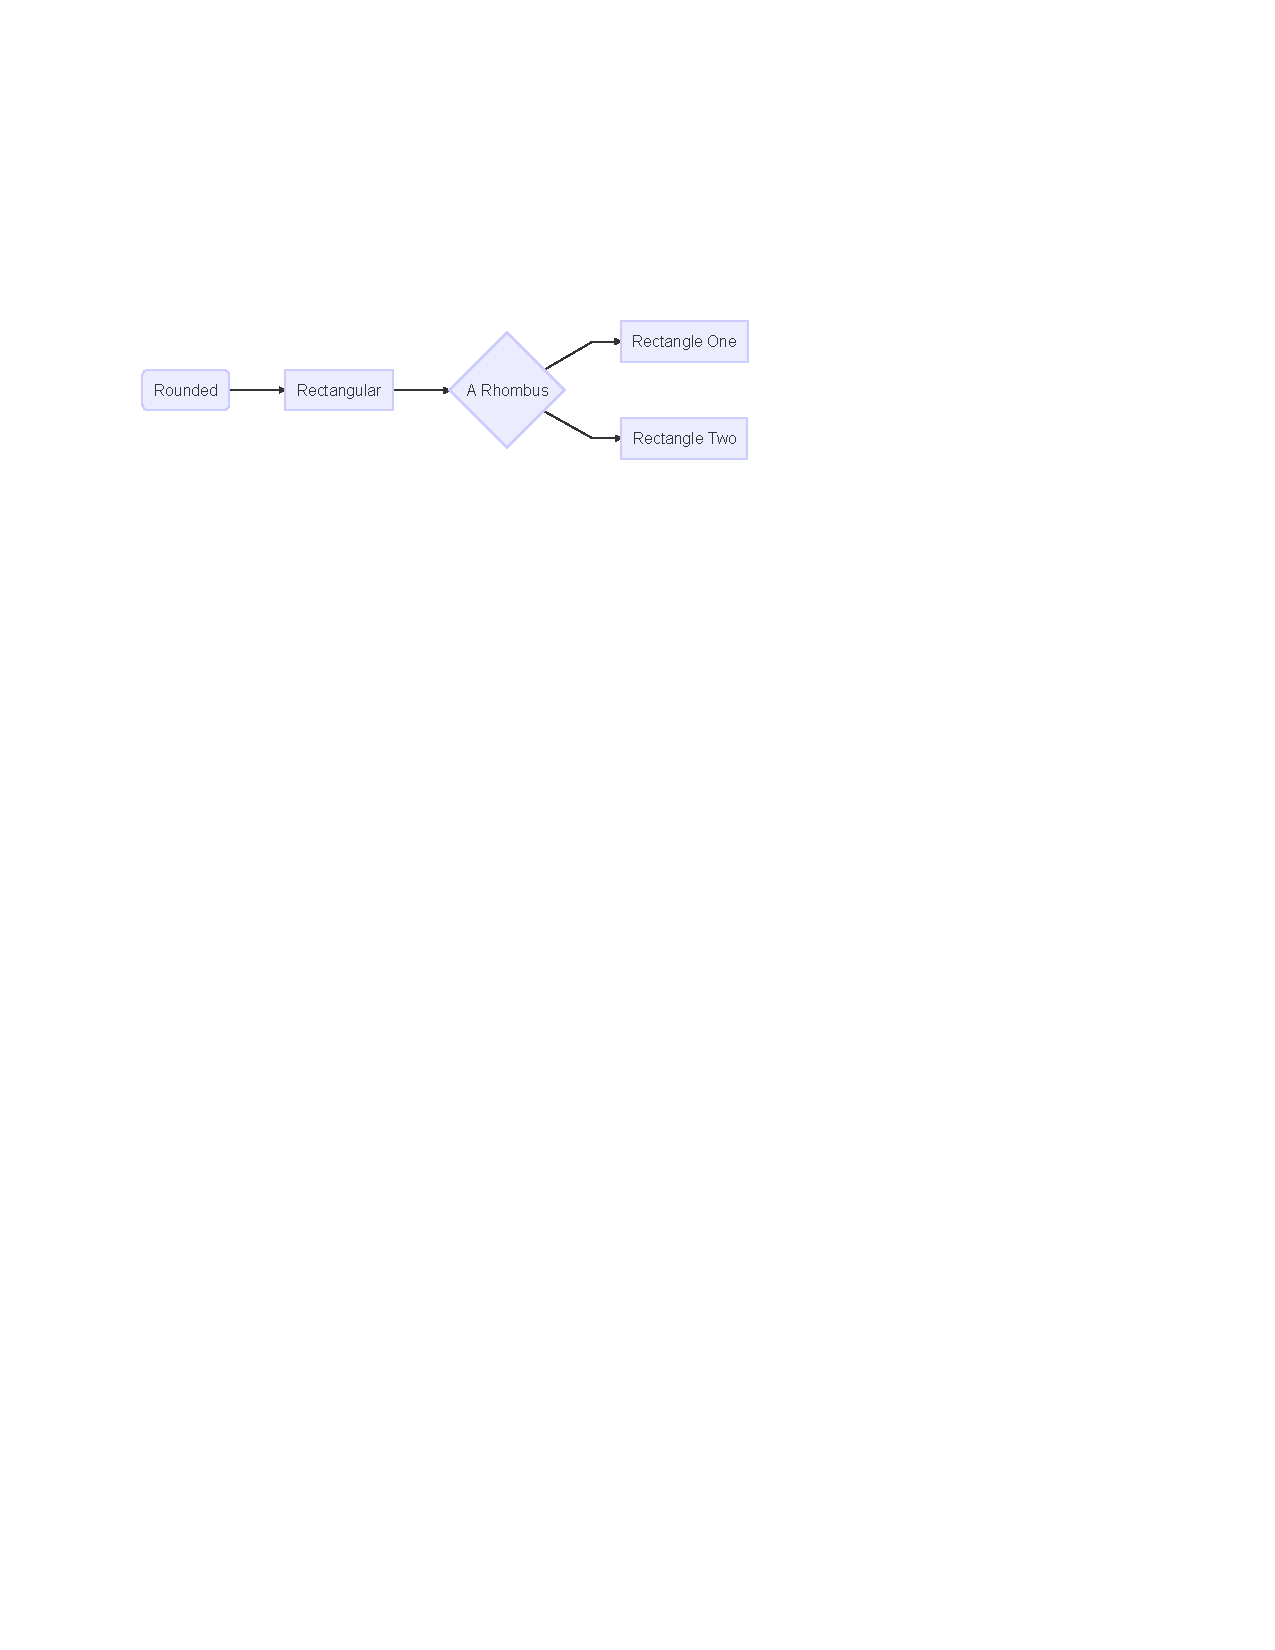
\includegraphics{./summary_files/figure-pdf/unnamed-chunk-4-6.pdf}

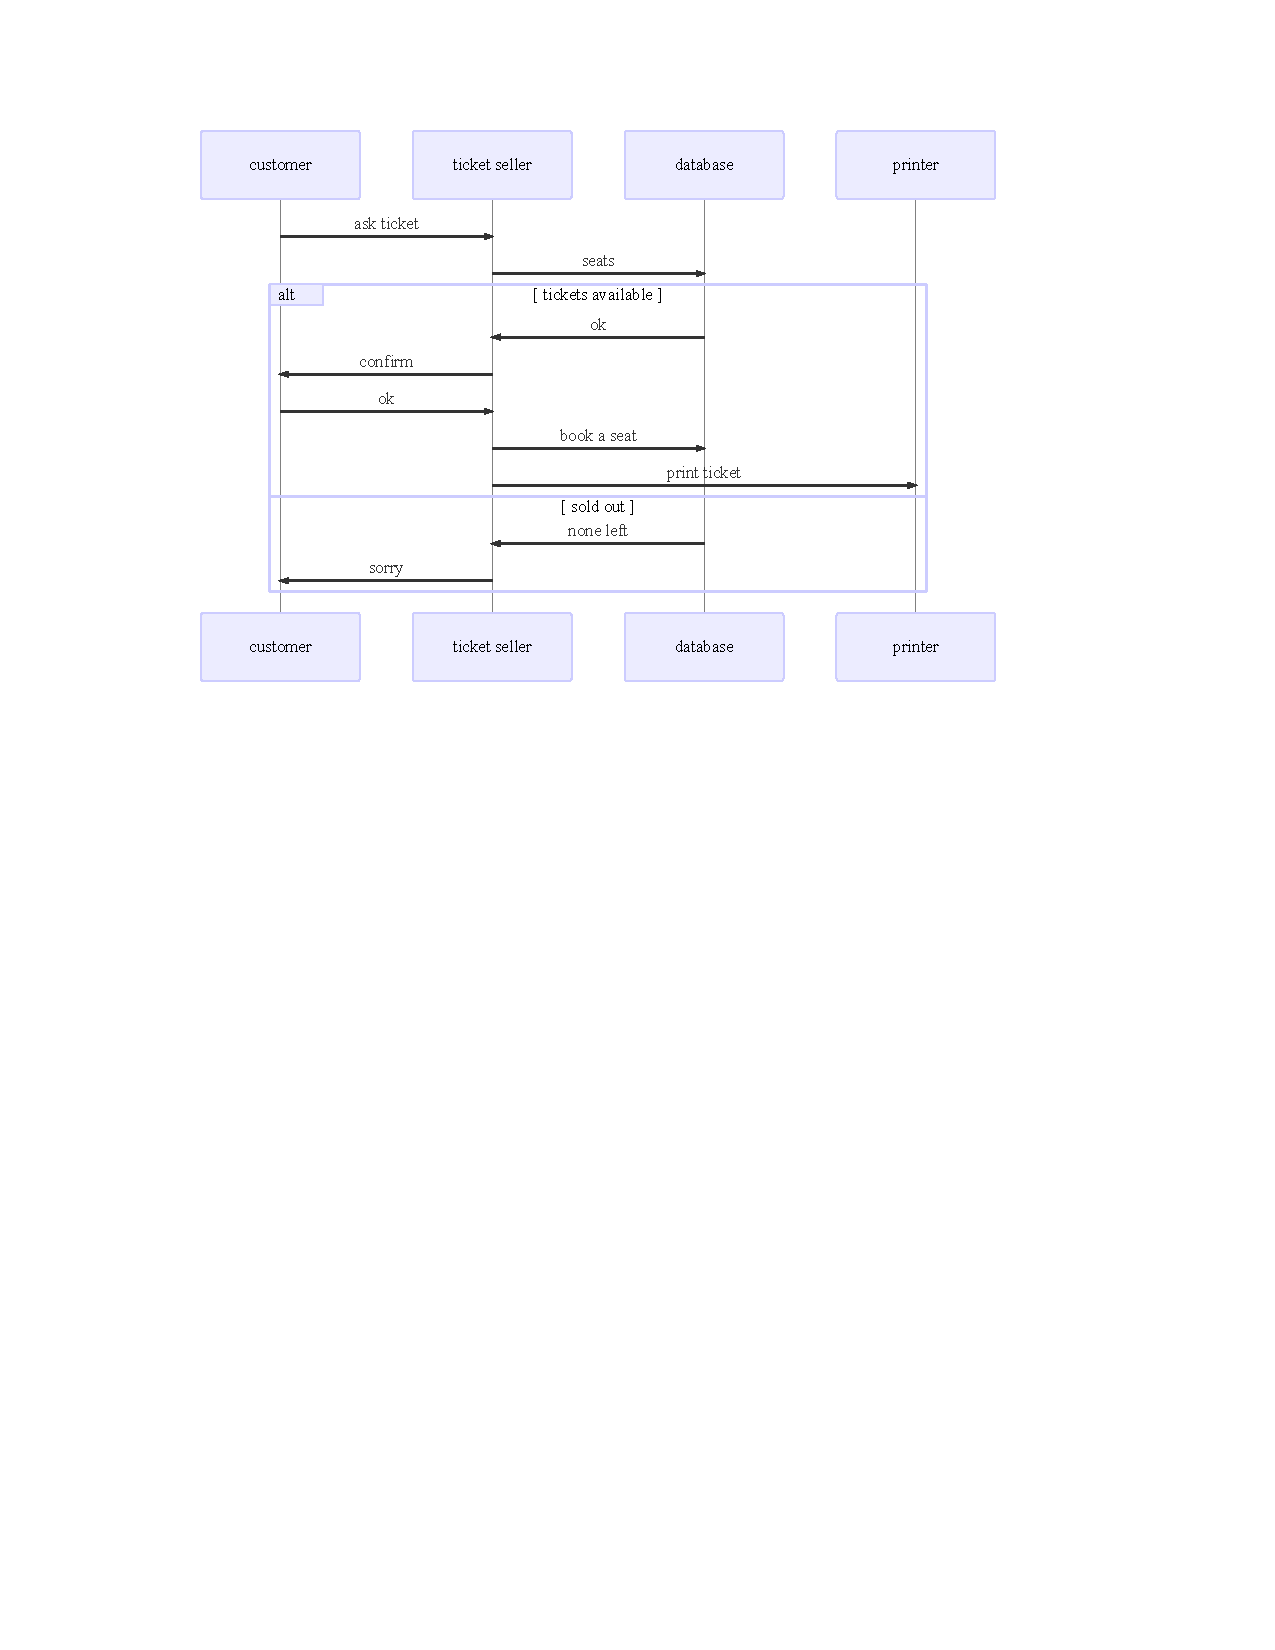
\includegraphics{./summary_files/figure-pdf/unnamed-chunk-5-1.pdf}

\bookmarksetup{startatroot}

\hypertarget{references}{%
\chapter*{References}\label{references}}
\addcontentsline{toc}{chapter}{References}

\markboth{References}{References}

\hypertarget{refs}{}
\begin{CSLReferences}{0}{0}
\end{CSLReferences}


\backmatter

\printindex

\end{document}
